\documentclass[12pt,a4paper]{article}
% page counting, header/footer
\usepackage{fancyhdr}
\usepackage{lastpage}
\usepackage[ngerman]{babel}
\usepackage{tikz}
\usetikzlibrary{decorations.markings}
\usepackage{amsmath}
\usepackage{amsfonts}
\usepackage{amssymb}
\usepackage{graphicx}
\usepackage[utf8]{inputenc}
\usepackage{hyperref}
\addtolength{\oddsidemargin}{-.525in}
\addtolength{\evensidemargin}{-.525in}
\addtolength{\textwidth}{1.5in}
\hypersetup{unicode=true,pdfborder={0 0 0 [0 0]}, linkcolor=blue}
\title{Lineare Algebra}
\author{Lucas Westermann \& Florian Scheibner}
\pagestyle{fancy}
\fancyhead{}
\fancyfoot{}
\fancyhead[L,L]{Lineare Algebra}
\fancyhead[R,R]{Lucas Westermann}
\fancyfoot[R,R]{Seite \thepage\ von \pageref{LastPage}}
\fancyfoot[L,L]{\hyperlink{contents}{Inhaltsverzeichnis}}
\renewcommand{\headrulewidth}{0.4pt}
\renewcommand{\footrulewidth}{0.4pt}
\setlength{\headheight}{16pt}
\newcommand{\alphabet}{\renewcommand{\labelenumi}{(\alph{enumi})}}
\newcommand{\numbers}{\renewcommand{\labelenumi}{(\arabic{enumi})}}
\newcommand{\romannum}{\renewcommand{\labelenumi}{(\roman{enumi})}}
\newcommand{\Romannum}{\renewcommand{\labelenumi}{(\Roman{enumi})}}
\newcommand{\R}{\mathbb{R}}
\newcommand{\K}{\mathbb{K}}
\newcommand{\Q}{\mathbb{Q}}
\newcommand{\Co}{\mathbb{C}}
\newcommand{\N}{\mathbb{N}}
\DeclareMathOperator{\sgn}{sgn}
\DeclareMathOperator{\id}{id}
\begin{document}
\maketitle
\pagebreak
\hypertarget{contents}{}
\tableofcontents
\pagebreak
\phantomsection
\section*{Literatur}
\addcontentsline{toc}{section}{Literatur}
\underline{Mathematik für Informatiker: } Teschl, Hackenberger \\
\underline{Lineare Algebra: } Beutelspacher, Fischer, Lang (auf Englisch), Stammbach.
\section{Grundlegendes}
\subsection{Mengen}
\subsubsection{Definition (Relation)}
Gegeben sein Mengen $X$ und $Y$.  Eine Teilmenge des kartesisches Produkt $X\times Y=\{(x,y):x\in X, y\in Y\}$ heißt \underline{Relation} ($R$) zwischen $X$ und $Y$; im Fall $X=Y$ spricht man von einer Relation auf $X$.  Ferner: $R^{-1}_1=\{(y,x)\in Y \in X: (x,y)\in R\}$ heißt \underline{Umkehrrelation}.
\subsubsection{Beispiel}
Die Menge $R_0=\{(x,y)\in X\in Y: y \mathrm{\ ist\ Hauptstadt\ von\ } x$ ist eine Relation zwischen der Menge $X$ aller Länder und $Y$ aller Städte. \\
\begin{center}
\includegraphics[scale=0.4]{1-1-2.jpg}
\end{center}
\subsubsection{Beispiel}
Mit den Mengen $X=\mathbb{R}$ $Y=[0,\infty)$ ist $R_1=\{(x,\left| x\right|) \in X\times Y, X\in X\}$ ist eine Relation mit der Umkehrrelation $R^{-1}=\{(\left| x\right|,x):x\in X\}$.\\
\begin{center}
\includegraphics[scale=0.4]{1-1-3.jpg}
\end{center}
\subsubsection{Beispiel}
Mit den Mengen $X=Y=\mathbb{R}$ ist $R_2=\{(x,y)\in X\times Y:x \leq y\}$
eine Relation $R^{-1}_{2}={(y,x):x\leq y}$ \\
 \begin{center}
\includegraphics[scale=0.4]{1-1-4.jpg}
\end{center}
\subsubsection{Beispiel}
Die Menge $R_3=\{(x,y)\in C\times C:x\ \mathrm{und\ } y \mathrm{\ haben\ gleichen\ Hersteller}\}$ ist eine Relation auf der Menge aller Computer $C$.
\subsubsection{Beschreibung (Gerichtete Graphen)}
Relation $R$ auf endlichen Mengen $X$ können alternative wie folgt dargestellt werden.  Man repr\"{a}sen\-tiert die Elemente von $X$ als Punkte in der Ebene (\underline{Knoten}) und verbindet $x,y\in X$ genau dann durch einen Pfeil (\underline{gerichtete Kante}), wenn $(x,y)\in R$.  Das paar $(X,R)$ heißt \underline{gerichteter Graph} oder \underline{Digraph}, z.B. $X=\{a,b,c\}$ $R=\{(a,b),(b,c),(c,d)\}$.\\
\begin{center}
\includegraphics[scale=0.4]{1-1-6.jpg}
\end{center}
$X=\{a,b,c\}$ $R=\{(b,a),(a,a),(c,c)\}$. \\
Eine Relation $R$ auf X heißt \\
\underline{reflexiv} $\Leftrightarrow (x,x)\in R$ für alle $x\in X$ \\
\underline{transitiv} $\Leftrightarrow (x,y)\in R \Rightarrow (x,z) \in R$ für alle $x,y,z\in X$\\
\underline{symmetrisch} $\Leftrightarrow (x,y)\in R$ für alle $x,y\in X$
\subsubsection{Beispiel}
Die Relation $R_2$ aus Beispiel 1.1.4 ist reflexiv, transitiv, aber nicht Symmetrisch.  Die Relation $R_3$ aus Beispiel 1.1.5 ist reflexiv, transitiv und symmetrisch.
\subsubsection{Definition (\"{A}quivalenzrelation)}
Eine Relation $A$ auf eine Menge $X$ heißt eine \underline{\"{A}quivalenzrelation}, falls sie reflexiv, transitiv und symmetrisch ist.  F\"{u}r ein Paar $(x,y)\in A$  Schreiben wir $x\mathtt{\sim} y$ und nennen $x$ und $y$ \"{a}quivalent.
\subsubsection{Beispiel}
\begin{enumerate}
\item Sei $X$ eine beliebige Menge.  Dann ist $\{(x,y)\in X\times X:x=y\}$ eine \"{A}quivalenzrelation (\underline{Identit\"{a}tsrelation}).
\item Ebenso ist das ganze Produkt $X\times X$ eine \"{A}quivalenzrelation (\underline{Allrelation}).
\item Die Relation $R_3$ aus Beispiel 1.1.5 ist eine \"{A}quivalenzrelation.  Mit ihr lassen sich Computer nach ihrem Hersteller klassifizieren.
F\"{u}r jedes $[x]:=\{y\in X:x \mathtt{\sim} y\}$ die von $X$ erzeugte \underline{\"{A}quivalenzklasse} und ein Element $y\in [x]$ heißt \underline{Repr\"{a}sentant} von $[x]$.
\end{enumerate}
\subsubsection{Beispiel}
\begin{enumerate}
\item F\"{u}r die Identit\"{a}tsrelation ist $[x]=\{x\}$ für alle $x\in X$.  Die Allrelation besitzt genau eine \"{A}quivalenzklasse $[x]=X$.
\item Im Beispiel 1.1.5 sind die \"{A}quivalenzklassen die Menge aller Hersteller.
\end{enumerate}

\subsection{Abbildungen}
$F\subseteq D\times B$.\\
\begin{center}
\includegraphics[scale=0.4]{1-2.jpg}
\end{center}
\subsubsection{Definition (Abbildungen, Funktion)}
Eine Relation F zwischen zwei nichtleeren Mengen $D$ und $B$ heißt \underline{Abbildung} oder \underline{Funktion} von $D$ nach $B$, falls f\"{u}r alle $x\in D$ gilt.\\
1) Es existiert ein $y\in B$ mit $(x,y) \in F$\\
2) Mit $y_1,y_2\in B$ folgt aus $(x,y_1) \in F$ und $(x,y_2)\in F$, dass $y_1=y_2$.\\
Die Menge $D$ heißt \underline{Definitionsbereich}  und $B$ \underline{Bildbereich} von $F$.  Im Fall $D=B$ spricht man von einer \underline{Abbildung auf $D$} oder um einer \underline{Selbstabbildung auf $D$}.
\subsubsection{Bemerkung}
Veranschaulicht man Funktionen auf (endlichen) Mengen $D$ als gerichtete Graphen (Beispiel 1.1.6), so geht von jedem Knoten genau eine Kante ab.
Anstelle der Notation $F \subseteq D \times B,\ (x,y)\in F$ schreibt man auch $f:D\rightarrow B, x\mapsto f(x)$ oder $y:=f(x)$
Mit einer weiteren nichtleeren Menge $C$ und einer Abbildung $g:B\rightarrow C$ ist die \underline{Verknüpfung (Komposition)} von $g$ und $f$ definiert als $g\circ f: D\rightarrow C, (g\circ f)(x):=g(f(x))$.  Im Fall von Abbildungen $f,g$ auf $D$ gilt i.A. $f\circ g\not = g\circ f$.
Statt einzelner Punkte $x\in D$ kann man auch Mengen $X\subseteq D$ abbilden: $f(X):=\{y\in B:$ es gibt ein $x\in X$ mit $y=f(x)\}$.  $f(X)$ heißt \underline{Bild} von $X$ unter $f$.  Das \underline{Urbild} einer Menge $Y\subseteq B$ ist definiert durch $f^{-1}(Y):=\{x\in D\ f(x)\in Y\}$.  Eine Abbildung $f:D\rightarrow B$ heißt \\
\underline{injektiv} $\Leftrightarrow f^{-1}(\{y\}$ enthält für alle $y\in B$ höchstens ein Element \\
\underline{surjektiv} $\Leftrightarrow f^{-1}(\{y\})$ enthält für alle $y\in B$ mindestens ein Element. \\
\underline{bijektiv} $\Leftrightarrow f^{-1}(\{y\})$ enthält für alle $y\in B$ genau ein Element. \\
Eine Abbildung $f:D\rightarrow B$ ist genau dann bijektiv, wenn sie injektiv und surjektiv ist.\\
\begin{center}
\includegraphics[scale=0.4]{1-2-2.jpg}
\end{center}
\subsubsection{Beispiel (identische Abbildung)}
Die \underline{identische Abbildung} auf eine Menge $D\not = \emptyset$ ist $id_D:D\rightarrow D,id_D(x):=x$. Sie ist bijektiv.
\subsubsection*{Beispiel}
Die Relation $R_0$ aus Beispiel 1.1.2 zwischen $X=\{Land\}$ und $Y=\{Stadt\}$ ist eine Funktion $r_o :X\rightarrow Y$ $r_0(Land):=$ Hauptstadt vom Land.  Ihr Bild ist $r_0(X)=\{$Hauptst\"{a}dte$\}$ und die Urbilder lauten:
\[r_0^{-1}(\{s\}) = \begin{cases}
\emptyset & \text{falls $s$ keine Hauptstadt},\\
\{l\}& \text{falls $s$ Hauptstadt von $l$}.
\end{cases}\]
Folglich ist $r_0$ injektiv, aber nicht surjektiv.  Betrachtet man die Menge aller Haupst\"{a}dte als Bildbereich von $r_0$, so ist diese Abbildung auch surjektiv.
\subsubsection{Beispiel}
Die Relation $R_1$ zwischen $\mathbb{R}$ und $[0,\infty )$ aus Beispiel 1.1.3 ist eine Abbildung und lässt sich schreiben als $r_1:\mathbb{R}\rightarrow [0,\infty ),\ r_1(x):=\left|x\right|$
F\"{u}r sie gilt $r_1(\mathbb{R}):=[0,\infty )$ und $r_1^{-1}(\{y\})=\{-y,y\}$ f\"{u}r alle $y\in [0,\infty )$.  Also ist $r_1:\mathbb{R}\rightarrow [0,\infty )$ surjektiv, aber nicht injektiv.  Betrachten wir $r_1$ mit ganz $\mathbb{R}$ als Bildbereich, so gilt $r_1^{-1}(\{y\})=\emptyset$ f\"{u}r $y<0$ und dann ist $r_1$ nicht mehr surjektiv.
\subsubsection{Beispiel (ASCII-Code)}
Der ASCII-Code zur Codierung alpha-numerischer Zeichen ist gegeben durch eine bijektive Abbildung $f:\{0,1,\cdots ,255\text{ bzw. $127$}\}\rightarrow \{$Zeichen$\}$.\\
Einfache Beispiele (etwa Beispiel 1.2.5) zeigen, dass die Umkehrrelation $F^{-1}$ einer Abbildung $F\subseteq D\times B$ bzw. $f:D\rightarrow B$ nicht unbedingt eine Abbildung ist.
\subsubsection{Definition (Umkehrabbildung)}
Eine Abbildung $f:D\rightarrow B$ heißt \underline{umkehrbar}, falls ihre Umkehrrelation $F^{-1}$ wieder eine Abbildung ist.  F\"{u}r letztere schreibt man $f^{-1}:B\rightarrow D$ und nennt sie \underline{Umkehrabbildung} von $f$.
\subsubsection{Bemerkung}
Mit einer umkehrbaren Abbildung $f:D\rightarrow B$ ist auch ihre Umkehrfunktion $f^{-1}:B\rightarrow D$ umkehrbar mit $f^{-1}\circ f = id_D$ und $f\circ f^{-1}=id_B$.
\subsubsection{Korollar}
Eine Abbildung $f:D\rightarrow B$ ist genau dann umkehrbar, wenn $f$ bijektiv ist.  F\"{u}r umgekehrtes $f$ existiert die Umkehrfunktion nur auf $f(D)$. \\
\underline{Beweis}: Hausaufgabe
\subsection{Matrizen}
Wir führen kurz die komplexen Zahlen $\mathbb{C}$ ein.  Darunter versteht man alle Paare $z=(x,y)$ reeller Zahlen $x,y\in \mathbb{R}$ mit der \underline{Addition}: \[z_1+z_2=(x_1+x_2,y_1+y_2)\] und der \underline{Multiplikation}: \[z_1\cdot z_2:=z_1z_2=(x_1x_2-y_1y_2,x_1y_2+x_2y_1)\] wobei $z_1=(x_1,y_1),z_2=(x_2,y_2)$ \\
Differenz und Quotient ergeben sich zu:
\[ z_1-z_2=(x_1-x_2,y_1-y_2)\]
\[\dfrac{z_1}{z_2} = \left(\dfrac{x_1x_2+y_1y_2}{x_2^2+y_2^2},\dfrac{x_2y_1-x_1y_2}{x_2^2+y_2^2}\right) \text{ falls } x_2^2+y_2^2\not = 0\]
Alternative Darstellung:
\[z=(x,y) = x+iy \text{ mit der Konvention } i^2=-1\]
Wobei $x$ der Realteil ($Rez=x$) ist und $y$ der Imaginärteil ($Imz=y$).\\
\begin{center}
\includegraphics[scale=0.4]{1-3.jpg}
\end{center}
Im Folgenden stehe $\mathbb{K}$ für eine der drei Mengen $\mathbb{Q}$ (rationalen Zahlen), $\mathbb{R}$ (reelle Zahlen) oder $\mathbb{C}$.
\subsubsection{Definition (Matrix)}
Eine $m\times m$-Matrize ist ein rechteckiges Schema von Zahlen $a_{ij}\in \mathbb{K}$ der Form \[A=(a_{i,j}) 1\leq i\leq m,1\leq j\leq m =\left( \begin{array}{cccc}a_{1,1}& a_{1,2}& \cdots & a_{1,m}\\ a_{2,1}& a_{2,2}& \cdots & a_{2,m} \\ \vdots & \vdots & \ddots & \vdots \\ a_{m,1}& a_{m,2}& \cdots & a_{m,m}\end{array}\right) \]
Der erste Index $i\in\{1,\cdots ,m\}$ nummeriert die $m$ \underline{Zeilen}, der zweite Index $j\in \{1,\cdots ,m\}$ die $m$ Spalten der Matrix $A$, das \underline{Element} $a_{ij}\in \mathbb{K}$ steht daher in der $i$-ten Zeile und der $j$-ten Spalte.  F\"{u}r die Menge aller solchen Matrizen schreiben wir $\mathbb{K}^{m\times m}$. Für eine \underline{quadratische Matrix} A gilt $m = n$ und die $a_{i,i}$ heißen \underline{Diagonalelement}.
\[A'=\left( \begin{array}{ccc}a_{1,1}& \cdots & a_{1,n}\\\vdots & \ddots & \vdots\\a_{m,1}& \cdots & a_{m,n}\end{array}\right)\]
\subsubsection{Beispiel ($n$ Tupeln, $m$-Spalten)}
Ein \underline{$n$-Tupel} $x=(x_1,\cdots ,x_n)$ von Zahlen $X$ aus $\mathbb{K}$ wird als $1\times m$-Matrix interpretiert.  Eine \underline{$m$-Spalte} $x=\left(\begin{array}{c}x_1\\\vdots \\x_m\end{array}\right)$
wird als $m\times 1$-Matrix verstanden, identifiziert durch $\mathbb{K}^m=k^{m\times 1}$.
\subsubsection{Kronecker-Symbol, Einheits- und Nullmatrixe)}
Wir definieren das \underline{Kronecker-Symbol} $S_{i,j}:=\begin{cases}1,i=j\\0,i\not= j\end{cases}$ und $I_m:=(S_{i,j})_{1\leq i,j\leq m}$ ist die \underline{Einheitsmatrix}.  Bei der Nullmatrix $0=(0)_{\substack{1\leq i\leq m\\1\leq j\leq n}}$ sind alle Elemente gleich $0\in \mathbb{N}$.
\subsubsection{Beispiel (Diagonal- und Dreieckmatrizen)}
Man nennt eine quadratische Matrix $A=(a_{i,j})_{1\leq i,j\leq n}$ \underline{diagonal} falls $a_{i,j}=0$ für $i\not=j$.  Wir schreiben dann $A=\left(\begin{array}{cccc}a_{1,1} & 0 & \cdot & 0\\ 0 & a_{2,2} &\cdot & 0\\ 0 &\cdot &\cdot & a_{n,n}\end{array}\right)=\text{diag}(a_{1,1},\cdot,a_{n,n})$.  Eine \underline{obere Dreiecksmatrix} ist quadratisch und erfüllt $a_{i,j}=0$ für $i>j$, wogegen eine \underline{untere Dreiecksmatrix} $a_{i,j}=0$ für $i<j$ erfüllt.  Sie sind von der Form: $A=\left(\begin{array}{cccc}a_{1,1} & a_{1,2} & \cdots & a_{1,n}\\ 0 & a_{2,2} & \cdots & a_{2,n}\\ \vdots & \vdots & \ddots &\vdots \\ 0 & \cdots & 0 & a_{n,n}\end{array}\right)$ bzw. $A=\left(\begin{array}{cccc}a_{1,1} & 0 & \cdots & 0\\a_{2,1} & a_{2,2} & \cdots & 0 \\ \vdots & \vdots & \ddots &\vdots \\ a_{n,1} & a_{n,2}  &\cdots & a_{n,n}\end{array}\right)$.\\
Mathematische Operationen für Matrizen:
\begin{itemize}
\item \underline{Skalare Multiplikation}: $\mathbb{K}\times \mathbb{K}^{m\times n} \rightarrow \mathbb{K}^{m\times n}, \alpha \cdot A= \alpha A=(\alpha a_{i,j})_{\substack{1\leq i\leq m \\ i\leq j\leq n}}$.  Wir schreiben $-A:=(-1)\cdot A$
\item \underline{Addition}: $+:\mathbb{K}^{m\times n}\times \mathbb{K}^{m\times n} \rightarrow \mathbb{K}^{m\times n},A+B=(a_{i,j}+b_{i,j})_{\substack{1\leq i\leq m \\ 1\leq j\leq n}}$.  Die Subtraktion lautet $A-B=A+(-B)$.
\item Genau für $m\times n$-Matrizen $A$ und $n\times p$-Matrizen $B$ lässt sich eine \underline{Multiplikation} erklären.  $\cdot : \mathbb{K}^{m\times n}\times \mathbb{K}^{n\times p}\rightarrow \mathbb{K}^{m\times p}$.  $A\cdot B=AB:=(\sum^n_{k=1} a_{i,k}b_{k,j})_{\substack{1\leq i\leq m\\1\leq j\leq p}}$. das Produkt ist also eine $m\times p$-Matrix.
\end{itemize}
\underline{Merke}: Das Produkt macht nur Sinn, falls die Spaltenzahl der ersten mit der Zeilenzahl der zweiten Matrix übereinstimmt.
\subsubsection{Bemerkung}
(1) Um Produkte von Matrizen $A\in \mathbb{K}^{m\times n}$ und $B\in \mathbb{K}^{n\times p}$ zum berechnen ergibt sich das Schema $\begin{array}{ccc} & | & B\\A & | & C\end{array} C=(\sum^{n}_{k=1} a_{i,k}b_{k,j})_{\substack{1\leq i\leq m\\1\leq j\leq p}}$\\
(2) Spezialfall: $A\in \mathbb{K}^{m\times m},x\in \mathbb{K}^m$ $Ax=\sum^{m}_{k=1}\left(\begin{array}{cc}a_{1,k}&x_{1}\\\vdots & \vdots \\ a_{m,k} & x_k\end{array}\right)$.
\subsubsection{Beispiel}
Das Produkt von $A=\left(\begin{array}{cc}0 & 1\\ 2 & 3\end{array}\right)$ und $B=\left(\begin{array}{cc}4 & 5 \\ 6 & 7\end{array}\right)$ lautet:
\[\begin{array}{c|cc} & \begin{matrix}4\\ 6\end{matrix} & \begin{matrix} 5\\ 7\end{matrix} \\ \hline \\0\ 1 & 0\cdot 4+1\cdot 6 & 5\cdot 0 + 1\cdot 7 \\ 2\ 3 & 2\cdot 4+6\cdot 3 & 2\cdot 5+7\cdot 3\end{array}\] also $C=AB=\left(\begin{array}{cc}6 & 7 \\ 26 & 31\end{array}\right)$.\\
Im Umgekehrter Reihenfolge gilt $BA=\left(\begin{array}{cc} 10 & 19 \\ 14 & 27\end{array}\right)$.  Daher ist das Produkt von Matrizen nicht kommutativ $AB\not= BA$.
\subsubsection{Beispiel}
(1) Für $A\in \mathbb{K}^{m\times n}$ gilt $I_m A=A=AI_m$\\
(2) Für $A=\left(\begin{array}{cc}0 & 1\\ 0 & 0\end{array}\right)$ und $B=\left(\begin{array}{cc}1 & 0\\ 0 & 0\end{array}\right)$ gilt $AB=0$, womit das Produkt von Matrizen nicht \underline{nullteilerfrei} ist, d.h. $AB=0$ kann gelten, ohne dass ein Faktor Null ist.\\
(3) Das Produkt von $\left(\begin{array}{ccc}0 & 1 & 2 \\ 3 & 4 & 5\end{array}\right)$ und $\left(\begin{array}{cc}6 & 7 \\ 8 & 9\end{array}\right)$ ist nicht definiert,
$\left(\begin{array}{cc}6 & 7 \\ 8 & 9\end{array}\right)\left(\begin{array}{ccc}0 & 1 & 2 \\ 3 & 4 & 5\end{array}\right) = \left(\begin{array}{ccc}21 & 34 & 47 \\ 27 & 44 & 61\end{array}\right)$ dagegen schon.
\subsubsection{Beispiel (RGB - Raum)}
Im RGB-Farbmodell werden Farben durch Tupel $(r,g,b)$ reeller Zahlen $r,g,b\in \mathbb{R}$ beschreiben: $(1,0,0)$ = rot, $(0,0,1)$ blau, $(1,1,0)$ gelb.  Alternativ: $YIQ$-Modell $(y,i,q)$. \\
Umrechnung $\left(\begin{array}{c}y\\i\\q\end{array}\right)=\left(\begin{array}{ccc}0.3 & 0.6 & 0.1\\ 0.6 & -0.3 & -0.3\\ 0.2 & -0.5 & 0.3\end{array}\right) \left(\begin{array}{c}r\\g\\b\end{array}\right)$.
\subsubsection{Beispiel (Inzedenzmatrix)}
Gerichtete Graphen ohne Schleifen (kein Knoten wird durch eine Kante mit sich selbst verbunden, siehe Bemerkung 1.1.6) mit den Knoten ${\hat{1},\cdots, \hat{m}}$ mit den Knoten ${1,\cdots ,m}$ lassen sich durch eine sogenannte \underline{Inzedenzmatrix} $A\in \mathbb{K}^{m\times n}$ beschreiben mit
\[a_{i,j}=\begin{cases}1,\text{ Von Knoten }\hat{1}\text{ geht die Kante }j\text{ aus.}\\ -1,\text{ ein Knoten }\hat{1}\text{ mündet die Kante }j\\0,\text{ Knoten }\hat{1}\text{ und Kante }j\text{ berühren sich nicht.}\end{cases}\]. 
\begin{tikzpicture}[node distance=2cm, auto]
\node (1) {$\hat{1}$};
\node (2) [right of = 1] {$\hat{2}$};
\node (3) [below of = 2] {$\hat{3}$};
\draw[decoration={markings,mark=at position 1 with {\arrow[ultra thick]{>}}},postaction={decorate}] (1) to node {1} (2);
\draw[decoration={markings,mark=at position 1 with {\arrow[ultra thick]{>}}},postaction={decorate}] (2) to node {3} (3);
\draw[decoration={markings,mark=at position 1 with {\arrow[ultra thick]{>}}},postaction={decorate}] (3) to node {2} (1);
\end{tikzpicture}
$A=\left(\begin{array}{ccc}1& -1 & 0\\ -1 & 0 & 1\\ 0 & 1 & -1\end{array}\right)$ \\
\begin{tikzpicture}[node distance=2cm, auto]
\node (1) {$\hat{1}$};
\node (2) [right of = 1] {$\hat{2}$};
\node (3) [below of = 2] {$\hat{3}$};
\draw[decoration={markings,mark=at position 1 with {\arrow[ultra thick]{>}}},postaction={decorate}] (1) to node {1} (2);
\draw[decoration={markings,mark=at position 1 with {\arrow[ultra thick]{>}}},postaction={decorate}] (1) to node {2} (3);
\end{tikzpicture} $A=\left(\begin{array}{cc}1 & 1\\ -1 & 0 \\ 0 & -1\end{array}\right)$ \\
\begin{tikzpicture}[node distance=2cm, auto]
\node (1) {$\hat{1}$};
\node (2) [right of = 1] {$\hat{2}$};
\node (3) [below of = 1, left of = 2] {$\hat{3}$};
\draw[decoration={markings,mark=at position 1 with {\arrow[ultra thick]{>}}},postaction={decorate}] (1) to node {1} (2);
\draw[decoration={markings,mark=at position 1 with {\arrow[ultra thick]{>}}},postaction={decorate}] (1.290) to node {2} (3.70);
\draw[decoration={markings,mark=at position 1 with {\arrow[ultra thick]{>}}},postaction={decorate}] (3.90) to node {3} (1.270);
\draw[decoration={markings,mark=at position 1 with {\arrow[ultra thick]{>}}},postaction={decorate},loop below] (3) to node {4} (3);
\end{tikzpicture} Nicht schleifen frei!
\subsubsection{Satz (Rechenregeln für Matrizen)}
Für Zahlen $\alpha \in \mathbb{K}$ und Matrizen $A\in \mathbb{K}^{m\times n},B\in\mathbb{K}^{m\times p}$ gilt das \underline{Distributiv-Gesetz}.  $A(B+C)=AB+AC$ für alle $C\in \mathbb{K}^{m\times p}$ und die \underline{Assoziativ-Gesetze} $(\alpha A)B=A(\alpha B), A(BC)=(AB)C$ für alle $C\in \mathbb{K}^{p\times q}$.
Beweis: Übung.
\subsection{Lineare Gleichungen}
\subsubsection{Definition (lineare Gleichung)}
Es seien $A\in \mathbb{K}^{m\times n}$ und $b\in \mathbb{K}^{m}$.  Dann bezeichnet man $(L_b)\ Ax=b$ als lineares \underline{Gleichungssystem} mit $m$ Gleichungen für die $n$ unbekannten $x_m\in \mathbb{K}$ oder kurz also \underline{lineare Gleichung} in $\mathbb{K}^m$.  $A$ heißt \underline{Koeffizientenmatrix} und $b$ \underline{Inhomogenität} von $(L_b)$.  Im Fall $b\not= 0$ nennt man $(L_b)$ \underline{inhomogen} und erhält andernfalls die \underline{homogene Gleichung}: $(L_0)\ Ax=0$.  Eine Lösung von $(L_b)$ ist ein Element $x\in \mathbb{K}^m$ mit $Ax=b$ und $L_b:=\{ x\in \mathbb{K}^m:Ax=b\}$ steht für die \underline{Lösungsmenge} von $(L_b)$.
\subsubsection{Bemerkung}
(1) Ausgeschrieben lautet $(L_b)$:\\$a_{1,1}x_1+a_{1,2}x_2+\cdots +a_{1,n}x_n = b_1\\a{2,1}x_1+a_{2,2}x_2+\cdots +a_{2,n}x_n = b_2\\\cdots \\a{m,1}x_1+a_{m,2}x_2+\cdots +a_{m,n}x_n=b_m$.\\Oder noch unübersichtlicher $\sum^n_{j=1} a_{i,j}x_j = b_i$ für $1\leq i\leq m$.\\
(2) $(L_b)$ hat stehts die \underline{triviale Lösung} $0\in \mathbb{K}^m$.  Inhomogene Gleichungen müssen nicht unbedingt lösbar sein: $0x=1$.\\
\subsubsection{Satz (Superpositionsprinzip)}
Es seien $x,y \in \mathbb{K}^n$ Lösungen von ($L_0$).  Dann ist auch $\alpha x+\beta y$ eine Lösung von ($L_0$), d.h. $\alpha x+\beta y\in L_0$ für alle $\alpha ,\beta \in \mathbb{K}$. \\
Beweis: Übung.
\subsubsection{Satz}
Ist $\hat{x}\in\mathbb{K}^n$ eine Lösung von ($L_b$) so gilt $L_b=\hat{x}+L_0$.  Hierbei: Für gegebene $x\in\mathbb{K}^n,A\subseteq \mathbb{K}^n$ ist $x+A:=\{y\in \mathbb{K}^n:\text{ es gibt ein }a\in A\text{ mit } y=x+a\}$\\
Beweis: Übung.
Nun: Explizite Lösung von ($L_b$)!\\
Besonders einfach, falls $A\in\mathbb{K}^{m\times n}$ diagonal ist gilt nämlich $a_{i,i}\not=0,1\leq i\leq n$, so besitzt ($L_b$) die eindeutige Lösung $x\in\mathbb{K}^n$ mit Elementen $X_1=\dfrac{b_i}{a_{i,i}}$ für $1\leq 1\leq n$ ist dagegen $d_{i,i}=0$ für ein $1\leq i\leq n$, so besitzt ($L_b$) unendlich viele Lösungen für $b_i=0$ und anderenfalls keine Lösung.\\
\underline{Allgemeinere Klasse}: Ein $A\in \mathbb{K}^{m\times n}$ ist in \underline{Zeilen-Stufen-Form} (ZSF) falls in jeder Zeile gilt:
\begin{enumerate}
\item[(1)] Beginnt sie mit $k$ Nullen, so stehen unter diesen Nullen lediglich weitere Nullen.\\
\item[(2)] Unter dem ersten Element $\not= 0$ stehen nur Nullen.\\
\end{enumerate}
Bei \underline{strenger ZSF } muss zusätzlich gelten:
\begin{enumerate}
\item[(3)] Über jedem ersten Element $\not= 0$ stehen nur Nullen\\
\end{enumerate}
\subsubsection{Beispiel}
\begin{enumerate}
\item[(1)] Obere Dreiecksmatrizen sind in ZSF, Diagonalmatrizen sogar in strenger ZSF.\\
\item[(2)] Bezeichnet $*$ ein Element $\not= 0$, so gilt:
\begin{itemize}
\item $\left(\begin{array}{ccc}* & * & *\\ * & * & *\\ 0 & 0 & *\end{array}\right)$,
$\left(\begin{array}{ccc}0 & * & *\\ 0 & * & *\\ 0 & * & *\end{array}\right)$,
$\left(\begin{array}{ccc}* & 0 & 0\\ * & * & 0\\ * & * & *\end{array}\right)$
sind nicht in ZSF.
\item $\left(\begin{array}{cccc}* & * & * & *\\ 0 & * & * & *\\ 0 & 0 & 0 & *\end{array}\right)$ ist in ZSF (aber nicht strenger ZSF).
\item $\left(\begin{array}{cccc}* & * & 0 & 0\\ 0 & 0 & * & 0\\ 0 & 0 & 0 & 0\end{array}\right)$ ist in strenger ZSF
\end{itemize}
\end{enumerate}
\subsubsection{Beispiel (Rückwärts-Substitution)}
Die inhomogene lineare Gleichung $(1.4b)\begin{cases}x_1+2x_2+3x_3+4x_4=1,\\ x_2+2x_3+3x_4=1,\\x_3+2x_4=1\end{cases}$ hat die Koeffizientenmatrix bzw. Inhomogenität $A=\left(\begin{array}{cccc}1 & 2 & 3 & 4 \\ 0 & 1 & 2 & 3\\ 0 & 0 & 1 & 2\end{array}\right), b=\left(\begin{array}{c}1\\ 1\\ 1\\\end{array}\right)$\\
\underline{Rückwärtssubstitution}: Aus der letzten Gleichung $x_3+2x_4=1$ sieht man, dass $x_4=t$ frei gewählt wenden kann, $t\in \mathbb{K}$.  Dies liefert $x_3=1-2t$.  Die bekannten variablen $x_3,x_4$ können in die zweite Gleichung von ($1.4b$) eingesetzt werden, also $x_2 = 1-2x_3-3x_4=t-1$ und analog liefert die erste Gleichung $x_1=1-2x_2-3x_3-4x_4=0$.  Die Lösungsmenge von ($1.4b$) ist also:\[L_b=\left\{\left(\begin{array}{c}0\\ t-1\\ 1-2t\\ t\end{array}\right)\in \mathbb{K}^4:t\in\mathbb{K}\right\} = \left(\begin{array}{c}0\\ -1\\ 1\\ 0\end{array}\right)+\mathbb{K}\left(\begin{array}{c}0\\ 1\\ -2 \\1\end{array}\right)\]
Die Lösungsmenge $L_b$ von ($L_b$) ändert sich nicht, wenn folgende Operationen auf ($1.4b$) angewandt werden:
\begin{itemize}
\item Vertauschen von Gleichungen
\item Multiplikation von Gleichungen mit $\alpha \in \mathbb{K}\\\{0\}$
\item Addition des $\alpha$-fachen der $k$-ten Gleichung zur $j$-ten.\\
Diese sind \underline{elementare Zeilentransformationen}.
\end{itemize}
ZIEL: Transformiere $A$ bzw. ($L_b$) auf ZSF mittels elementarer Zeilentransformationen.  Systematisch: Gauß Algorithmus.\\
Zu seiner Beschreibung gehen wir davon aus, dass die erste Spalte von $A$ von $0$ verschieden ist (anderenfalls sind $x_1,\cdots ,x_n$ umzunummerieren).  Ohne Sonderfälle zu berücksichtigen gilt:
\begin{enumerate}
\item Ordne die Gleichungen in ($1.4a$) so an, dass $a_m\not= 0$.  In der gängigen Notation schreibt man nun ($1.4b$) als $\begin{array}{cccc|c}a_{1,1} & a_{1,2} & \cdots & a_{1,n} & b_1\\a_{2,1} & a_{2,2} & \cdots & a_{2,n} & b_2\\\vdots & \vdots & \ddots &\vdots &\vdots \\a_{m,1} & a_{m,2} & \cdots & a_{m,n} & b_m\end{array}$
\item Subtrahiere von der $i$-ten Gleichung, $2\leq i\leq m$ in ($1.4a$) das $\dfrac{a_{i,1}}{a_{1,1}}$-fache der ersten Gleichung: 
\[\begin{array}{cccc|c}a_{1,1} & a_{1,2} & \cdots & a_{1,n} & b_1\\0 & a_{2,2}^{(1)} & \cdots & a_{2,n}^{(1)} & b_2^{(1)}\\ \vdots &\vdots &\ddots &\vdots &\vdots \\0 & a_{m,2}^{(2)} & \cdots & a_{m,n}^{(1)} & b_m^{(1)}\end{array} \begin{cases}a_{1,1}x_1+\cdots + a_{1,n}x_n=b_1 \\ A^{(1)}x^{(1)} = b^{(1)}\end{cases}\]
mit $A^{(1)}\in\mathbb{K}^{(m-1)\times (n-1)},b\in \mathbb{K}^{m-1}$.
\item Transformiere $A^{(1)}x^{(1)} = b^{(1)}$ entsprechend und fahre sukzessive fort, bis (idealerweise) eine Dreiecks- oder ZSF entstanden ist.
\item Löse das resultierende System durch Rückwärts-Substitution.
\end{enumerate}
\subsubsection{Beispiel}
Als Kurzschreibweise für \[(1.4d)\begin{cases}x_1+2x_2+3x_3=0\\ 4x_1+5x_2+6x_3=0\\ 7x_1+8x_2+9x_3=0\end{cases}\]
\[\begin{array}{ccc|c}1 & 2 & 3 & 0\\ 4 & 5 & 6 & 0\\ 7 & 8 & 9 & 0\end{array} \begin{array}{c} \\ II - 4I\\ II-7I\end{array} \Leftrightarrow \begin{array}{ccc|c}1 & 2 & 3 & 0\\ 0 & -3 & -6 & 0\\ 0 & -6 & -12 & 0\end{array} \begin{array}{c} \\ (-\frac{1}{3})\\ III-2II\end{array} \Leftrightarrow \begin{array}{ccc|c}1 & 2 & 3 & 0\\ 0 & 1 & 2 & 0\\ 0 & 0 & 0 & 0\end{array}\]
Damit ist ($1.4d$) äquivalent zu $\begin{cases}x_1+2x_2+3x_3=0\\ x_2+2x_3=0\end{cases}$\\
Rückwärts-Substitution: Wähle $x_3=t$ mit $t\in\mathbb{K}$ und es folgt $x_2=-2x_3=-2t,x_1=-2x_2+3x_3=t$.  Die Lösungsmenge von ($1.4d$) ergibt sich zu:
\[ L_0=\left\{\left(\begin{array}{c}1\\ -2\\ 1\end{array}\right) \in \mathbb{K}^3:t\in\mathbb{K}\right\} = \mathbb{K}\left(\begin{array}{c}1\\ -2\\ 1\end{array}\right)\]
\subsubsection{Satz}
Hat ($L_0$) weniger Gleichungen als Unbekannte, also $m<n$, so besitzt sie unendlich viele Lösungen.
\underline{Beweis}:
\renewcommand{\labelenumi}{\Roman{enumi}.}
\begin{enumerate}
\item Man zeigt (*) ($L_0$) hat eine nichttriviale Lösung.
\item Da ($L_0$) nach Schritt (I) eine Lösung $x\not= 0$ besitzt ist nach dem superpositionsprinzip aus Satz 1.4.3 auch jeder $tx,t\in \mathbb{K}$, eine Lösung \#.
\end{enumerate}
\subsubsection{Satz}
Besitzt ($L_b$) genauso viele Gleichungen wie Unbekannte, also $m=n$, so gilt:
\renewcommand{\labelenumi}{(\alph{enumi})}
\begin{enumerate}
\item Ist $L_0=\{0\}$, so besitzt ($L_b$) genau eine Lösung.
\item Besitzt ($L_0$) eine nichttriviale Lösung, so existieren entweder keine oder unendlich viele verschiedene Lösungen von ($L_b$)
\end{enumerate}
\underline{Beweis}:
\begin{enumerate}
\item Wie gehen mittels vollständiger Induktion vor.\\
Für $n=1$ gilt die Behauptung offenbar.  Im Induktionsschritt gelte (a) für $n-1$.  Da ($L_0$) nur die triviale Lösung hat gilt $A\not= 0$.  Durch Umnummerieren erreichen wir $a_{1,1}\not= 0$.  Dann wird zur $i$-ten Gleichung, $2\leq i$, in ($1.4a$) das $-\frac{a_{i,1}}{a_{1,1}}$-fache der ersten Gleichung addiert:
\[(1.4f)\begin{cases}a_{1,1}x_1+\cdots +a_{1,n}x_n = b_1\\ A^*=\left[\begin{array}{c}x_2\\ \cdots \\ x_n\end{array}\right]= b^*\end{cases} \text{ mit }A^*\in \mathbb{K}^{(n-1)\times (m-1)}, b^*\in \mathbb{K}^{n-1} \]
Beweis: \\
Wir wissen:
\begin{enumerate}
\item Die homogene Gleichung $A^*x^* = 0$ hat nur die triviale Lösung, denn sonst hätte ($L_0$) eine nicht triviale Lösung.  Das Teilsystem $A^*x^* = b^*$ besitzt nach Induktionsannahme genau eine Lösung $x^*$ mit Elementen $x_2,\cdots ,x_m$.  Durch Einsetzten in die erste Gleichung in ($1.4f$) folgt ein eindeutiger Wert $x_1$ und die Lösung von ($L_b$) in eindeutiger Weise.
\item Es sei $\hat{x}$ eine Lösung von ($L_b$) und $x$ eine nichttriviale Lösung von ($L_o$).  Dann liefern die Sätze $1.4.3$ und $1.4.4$, dass $\hat{x}+\alpha x$ die Gleichung löst für jedes $\alpha \in \mathbb{K}$.  In diesem Fall hat ($L_b$) unendlich viele Lösungen.  Die einzige verbleibende Möglichkeit ist, dass ($L_b$) keine Lösung besitzt.
\end{enumerate}
\end{enumerate}

\section{Lineare Räume}
\subsection{Algebraische Strukturen}
Bezeichnet $M\not=\emptyset$ eine Menge und $F(M)$ die Menge aller Selbstabbildungen auf $M$, so kann die Komposition $\circ$ als Abbildung $\circ : F(M)\times F(M) \rightarrow F(M)$ interpretiert werden - man spricht von einer \underline{Verknüpfung}.
\subsubsection{Definition (Gruppe)}
Eine \underline{Gruppe} $(G,\cdot)$ ist eine nichtleer Menge $\mathbb{G}$ mit einer Veknüpfung $\cdot:\mathbb{G}\times\mathbb{G} \rightarrow \mathbb{G}$ mit den Eigenschaften:
$(G_1) \cdot$ ist \underline{Assoziativ}, d.h. $a\cdot(b\cdot c)=(a\cdot b)\cdot c$ für $a,b,c\in \mathbb{G}$\\
$(G_2)$ es existiert ein \underline{neutrales Element} $e\in\mathbb{G}$ mit $a\cdot e=a=e\cdot a$ für $a\in\mathbb{G}$\\
$(G_3)$ zu jedem $a\in\mathbb{G}$ existiert ein \underline{inverses Element} $a^{-1}\in \mathbb{G}$ mit $a\cdot a^{-1}=a^{-1}\cdot a=e$ für $a\in \mathbb{G}$\\
Bei einer kommutativen oder Abel'scher Gruppe gilt ferner $(G_4) a\cdot b=b\cdot a$ für alle $a,b\in \mathbb{G}$.  Für eine \underline{Halbgruppe} müssen nur $(G_1)$ und $(G_2)$ gelten.
\subsubsection{Bemerkung}
\renewcommand{\labelenumi}{(\arabic{enumi})}
\begin{enumerate}
\item Das neutrale Element $e\in\mathbb{G}$ ist eindeutig: In der Tat, bezeichnen $e_1,e_2\in\mathbb{G}$ zwei neutrale Elemente, so folgt nach $(G_2)$ ist: $e_2=e_1\cdot e_2$ und $e_1\cdot e_2=e_1$, also $e_1=e_2$
\item Zu gegebenem $a\in\mathbb{G}$ ist auch das inverse Element $a^{-1}\in\mathbb{G}$ eindeutig.  Für inverse Element $a_1^{-1},a_2^{-1}$ von $a$ gilt nämlich
\[a_1^{-1}\stackrel{(G_2)}{=}a_1^{-1}\cdot e\stackrel{(G_3)}{=}a_1^{-1}\cdot(a\cdot a_2^{-1})\stackrel{(G_1)}{=}(a_1^{-1}\cdot a)\cdot a_2^{-1}\stackrel{(G_3)}{=}e\cdot a_2^{-1}\stackrel{(G_2)}{=}a_2^{-1}\]
\item Entsprechend $e=e^{-1}$, $a=(a^{-1})^{-1}$
\end{enumerate}
\subsubsection{Bemerkung (Potenzen)}
Die Potenzen $a^n\in \mathbb{G}$ eines $a\in\mathbb{G}$ (G ist eine multiplikative Halbgruppe) sind rekursiv erklärt durch $a^0:=e, a^{n+1}:=a\cdot a^n$ für alle $n\in\mathbb{N}_0$.  In einer Gruppe setzen wir $a^n:=(a^{-n})^{-1}$ für $n<0$.
\subsubsection{Beispiel}
\begin{enumerate}
\item $(\mathbb{Z},+)$ ist eine kommutative additive Gruppe mit neutralen Element $0$ und dem zu $a\in\mathbb{Z}$ inverses Element $-a$.  Dagegen ist $(\mathbb{Z},\cdot )$ keine Gruppe, denn das multiplikative Inverses lässt sich innerhalb von $\mathbb{Z}$ nicht erklären.  Ebenso ist $(\mathbb{N},+)$ keine (additive) Gruppe.
\item Es sei $\mathbb{K}\in \{\mathbb{Q},\mathbb{R},\mathbb{C}\}$. Dann ist $(\mathbb{K},+)$ eine kommutative additive Gruppe mit neutralem Element $0$ und $-a$ als zu $a$ Inversen.  Auch $(\mathbb{K}\setminus \{0\},\cdot )$ ist eine kommutative multiplikative Gruppe mit neutralem Element $1$ und dem zu $a$ inversen Element $\frac{1}{a}$.
\item Mit $\mathbb{K}\in\{\mathbb{Z},\mathbb{Q},\mathbb{C}\}$ bilden die Matrizen $(\mathbb{K}^{m\times n},+)$ eine kommutative additive Gruppe mit neutralem Element $0$ und den Inversen $-A$ zu $A$.  Die quadratischen reellen rationalen oder komplexen Matrizen $(\mathbb{K}^{m\times n}\setminus \{0\},\cdot)$ bilden keine Gruppe, da etwa diag$(1,0)\not= 0$ kein Inverses besitzt.
\end{enumerate}
\addtocounter{subsubsection}{1}
\subsubsection{Beispiel (modulo)}
Es sei $p\geq 2$ eine ganze Zahl und $\mathbb{Z}_p:=\{0,\cdots ,p-1\}$.  Für beliebige $a,b\in\mathbb{Z}$ gibt es vermöge der Division mit Rest eindeutige $m\in\mathbb{Z}$ und $k\in\mathbb{Z}_p$ mit $a+b=mp+k$ wir schreiben dann $k=a+b$ mod $p$ oder $k=:a+_p b$.  Dann ist $(\mathbb{Z}_p,+_p)$ eine kommutative Gruppe mit dem neutralem Element $0$.
\subsubsection{Beispiel (symmetrische Gruppe)}
Es sei $M$ eine nichtleere Menge und $S(M)$ bezeichnet alle bijektiven Selbstabbildungen $f:M\rightarrow M$.  Dann ist die \underline{symmetrischen Gruppe} $(S(M),\circ )$ eine i.A. nicht-kommutative Gruppe mit id$_m$ als neutralem Element und $f^{-1}:M\rightarrow M$ als inversen Element zu $f$.  Im Fall $M=\{1,\cdots ,n\}$ schreiben wir $S_n:=S(\{1,\cdots ,n\})$.  Die Menge aller nicht-notwendig bijektiven Selbstabbildungen $F(M)$ ist dagegen eine Halbgruppe bezüglich $\circ$.
\subsubsection{Korollar (Rechnen in Gruppen)}
Für alle $a,b,c\in\mathbb{G}$ gilt $(a\cdot b)^{-1}=b^{-1}\cdot a^{-1}$, wie auch $a\cdot b=a\cdot c\Rightarrow b=c,a\cdot b=e\Rightarrow a=b^{-1}$.\\
Beweis:\\
Es seien $a,b,c\in\mathbb{G}$.  Wir zeigen zunächst, dass $b^{-1}\cdot a^{-1}$ das inverse Element von $a\cdot b$ ist.  Dazu 
\[(b^{-1}\cdot a^{-1})\cdot(a\cdot b)\stackrel{(G_1)}{=} b^{-1}\cdot(a^{-1}\cdot(a\cdot b\cdot))\stackrel{(G_1)}{=}b^{-1}\cdot((a^{-1}\cdot a)\cdot b)\stackrel{(G_3)}{=} b^{-1}\cdot(e\cdot b)\stackrel{(G_2)}{=}b^{-1}\cdot b\stackrel{(G_3)}{=}e\]
und entsprechend $(a\cdot b)\cdot(b^{-1}\cdot a^{-1})=e$.  Die erste Implikation ergibt sich nach Voraussetzung durch 
\[b\stackrel{(G_2)}{=}e\cdot b\stackrel{(G_3)}{=}(a^{-1}\cdot a)\cdot b\stackrel{(G_1)}{=}a^{-1}+(a\cdot b)=a^{-1}\cdot(a\cdot c)\stackrel{(G_1)}{=}(a^{-1}\cdot a)\cdot c\stackrel{(G_3)}{=}e\cdot c\stackrel{(G_2)}{=}c\]
Die verbleibende Implikation sei den Leser überlassen.
\subsubsection{Definition (Körper)}
Ein \underline{Körper} $(\mathbb{K},+,\cdot )$ ist eine Menge $\mathbb{K}$ mit mindestens zwei Elementen versehen.\\Mit den \underline{arithmetischen Operationen} $+: \mathbb{K}\times\mathbb{K}\rightarrow \mathbb{K}$ (\underline{Addition}) und $\cdot : \mathbb{K}\times\mathbb{K}\rightarrow \mathbb{K}$(\underline{Multiplikation}).\\
$(\mathbb{K}_1) (\mathbb{K},+)$ ist eine kommutative Gruppe mit neutralem Element $0$ und den zu $\alpha\in\mathbb{K}$ inversen Element $-\alpha$, d.h. für alle $\alpha ,\beta ,\gamma\in\mathbb{K}$ gilt:\\
\begin{align*}
(\mathbb{K}_1^1) & \alpha +(\beta + \gamma )= (\alpha + \beta)+\gamma \\
(\mathbb{K}_1^2) & \alpha + 0 = 0 + \alpha = \alpha \\
(\mathbb{K}_1^3) & \alpha \cdot -\alpha = -\alpha \cdot \alpha = 0 \\
(\mathbb{K}_1^4) & \alpha + \beta = \beta + \alpha
\end{align*}
($\mathbb{K}_2$) ($\mathbb{K}\setminus \{0\},\cdot$) ist eine kommutative Gruppe mit neutralem Element $1$ und zu $\alpha\in \mathbb{K}$ Inversem $\frac{1}{\alpha}$, d.h. es gilt für $\alpha ,\beta ,\gamma \in \mathbb{K}\setminus \{0\}$.
\begin{align*}
(\mathbb{K}_2^1) & \alpha \cdot (\beta \cdot \gamma ) = (\alpha \cdot \beta )\cdot \gamma\\
(\mathbb{K}_2^2) & \alpha \cdot 1 = 1\cdot\alpha = \alpha \\
(\mathbb{K}_2^3) & \alpha \cdot \frac{1}{\alpha} = \frac{1}{\alpha}\cdot\alpha = 1 \\
(\mathbb{K}_2^4) & \alpha \cdot \beta = \beta \cdot \alpha
\end{align*}
($\mathbb{K}_3$) es gelten die Distributivgesetze $\alpha (\beta +\gamma )=\alpha \cdot \beta + \alpha \cdot \gamma$, $(\alpha + \beta ) \cdot \gamma = \alpha\gamma + \beta\gamma$ für alle $\alpha ,\beta ,\gamma \in \mathbb{K}$.  Üblich $\alpha\beta :=\alpha \cdot \gamma$.  Subtraktion als $\alpha - \beta := \alpha + (-\beta )$.  Division $\frac{\alpha}{\beta} := \alpha \cdot \frac{1}{\beta}$.
\subsubsection{Beispiel}
$\mathbb{Q},\mathbb{R},\mathbb{C}$ sind Körper bzgl. $+,\cdot$
\subsubsection{Beispiel (Restklassenkörper modulo $p$)}
Mit einer gegebenen Primzahl $p\in\mathbb{N}$ definieren wir die Mengen $\mathbb{Z}_p := \{0,\cdots ,p\}$.  Dann gibt für beliebige $\alpha ,\beta \in \mathbb{Z}_p$ eindeutige Zahlen $m,n\in\mathbb{Z}$ und $k,l\in\mathbb{Z}_p$ derart, dass 
\[\alpha + \beta = m\cdot p+k\]
\[\alpha\cdot\beta = np+l \text{ Divison mit Rest.}\]
\[\text{Addition: }\alpha+_p \beta := k\]
\[\text{Multiplikation: }\alpha \cdot_p \beta := l\text{ (2.1a)}\]
$(\mathbb{Z}_p,+_p,\cdot_p)$ ist Körper, der sogenannten Restklassenkörper modulo $p$.
\[\mathbb{Z}_2: \begin{array}{c|cc}+_2 & 0 & 1\\ \hline\\ 0 & 0 & 1 \\ 1 & 1 & 0\end{array} \]
\[\begin{array}{c|cc}\cdot_2 & 0 & 1\\ \hline \\ 0 & 0 & 0 \\ 1 & 0 & 1\end{array} \]
\[\mathbb{Z}_3: \begin{array}{c|ccc}+_3 & 0 & 1 & 2\\ \hline \\ 0 & 0 & 1 & 2\\ 1 & 1 & 2 & 0\\2 & 2 & 0 & 1\end{array} \]
\[\begin{array}{c|ccc}\cdot_3 & 0 & 1 & 2\\ \hline \\ 0 & 0 & 0 & 0\\ 1 & 0 & 1 & 2\\2 & 0 & 2 & 1\end{array} \]
\subsubsection{Korollar}
Ist ($\mathbb{K},+,\cdot $) ein Körper, so gilt für alle $\alpha ,\beta ,\gamma \in \mathbb{K}$, dass
\begin{align*}
0\cdot \alpha &= \alpha \cdot 0 = 0, & \beta\cdot (-\alpha ) = -(\beta \cdot \alpha ) = (-\beta )\cdot \alpha &(2.1b)\\
(-1)\cdot \alpha &= -\alpha , & (-\alpha )\cdot (-\beta ) = \alpha\cdot\beta &(2.1c)
\end{align*}
Und ferner die Implikation $\alpha\cdot\beta = 0 \rightarrow \alpha = 0$ oder $\beta = 0$.
\subsubsection{Bemerkung}
Es gilt $1\not=0$, da die Annahme $1=0$ folgenden Widerspruch impliziert: Da $\mathbb{K}$ mindestens $2$ Elemente enthält, gibt es ein $\alpha\in\mathbb{K}, \alpha\not= 0$ mit:
\[\alpha \stackrel{(\mathbb{K}_2^2)}{=} \alpha \cdot 1 = \alpha \cdot 0 \stackrel{(2.1b)}{=} 0\]
Daher ist der Restklassenkörper modulo $2\ \mathbb{Z}_2$ der kleinste Körper.
\subsubsection{Beweis}
Wähle ein $\alpha ,\beta ,\gamma \in\mathbb{K}$. Es gilt $0\cdot \alpha \stackrel{(\mathbb{K}_1^2)}{=} (0+0)\cdot \alpha \stackrel{(\mathbb{K})}{=} 0\alpha + 0\alpha$ mittels Korollar 2.1.8 ($+,a=b=0$ und $c=0$) folgt $0\cdot \alpha = 0$, kommutativ liefert $\alpha 0 = 0$. Aus dieser Behauptung resultiert 
\[(-\beta )\alpha +\beta\alpha \stackrel{(\mathbb{K}_3)}{=} (-\beta + \beta)\alpha = 0\cdot \alpha = 0\]
mit Korollar 2.1.8 ($+,a=(-\beta )\alpha ,b=\beta\alpha$).  Dies liefert $-(\beta\alpha )=(-\beta )\alpha$ und $\beta (-\alpha )=-(\beta\alpha )$.  Die Beziehung $(-1)\alpha = -\alpha $ resultiert aus dem eben gezeigten $\beta = 1$ und 
\[(-1)\alpha = 1\cdot (-\alpha ) \stackrel{\mathbb{K}_2^2)}{=} -\alpha .\]
$2.1c$ ergibt sich mit Bemerkung $2.1.2(3)$ aus 
\[(-\alpha ) (-\beta )\stackrel{2.1b}{=}-(\alpha (-\beta )) \stackrel{2.1b}{=} -(-(\alpha\beta )) = \alpha\beta =0 \]
Annahme: $\alpha \not=0$ und $\beta\not=0$ dann $1\stackrel{\mathbb{K}_2^3)}{=}\frac{1}{\beta} \cdot \frac{1}{\alpha} \cdot \alpha\cdot\beta \stackrel{2.1b}{=} 0$
\subsection{Vektorräume}
\subsubsection{Definition (linearer Raum, Vektorraum)}
Es sei $\mathbb{K}$ ein Körper.  Ein Vektorraum oder linearer Raum $(X,+,\cdot )$ (über $\mathbb{K}$) ist eine nichtleere Menge $X$ mit arithmetische Operationen:
\begin{enumerate}
\item Addition $+:\ X\times X\rightarrow X$ derart, dass $(X,+)$ eine kommutative Gruppe mit neutralem Element $0$ oder Nullvektor.
\item Skalare Multiplikation $\cdot :\mathbb{K}\times X\rightarrow X$ derart, dass für alle $\alpha ,\beta \in \mathbb{K}$ und $x,y\in X$ gilt:
\begin{align*}
(V_1)&\ \alpha (x+y) = \alpha x+\alpha y \text{ Distributiv Gesetz}\\
(V_2)&\ (\alpha +\beta ) \cdot x = \alpha x + \beta x \text{ Distributiv Gesetz} \\
(V_3)&\ (\alpha\beta )\cdot x = \alpha \cdot (\beta \cdot x) \text{ Assoziativ Gesetz}\\
(V_4)&\ 1\cdot x = x
\end{align*}
Die Elemente aus $\mathbb{K}$ heißen Skalare und $X$ heißen Vektoren.
\end{enumerate}
Konventionen: $\alpha x := \alpha\cdot x$  $x-y:=x+(-y)$
\subsubsection{Beispiel}
Es sei ($\mathbb{K},+,\cdot $) ein Körper.\\
($0$) Der triviale Raum $\{0\}$ der nur die $0$ enthält.\\
($1$) Weiter ist $\mathbb{K}$ ein Vektorraum über sich selbst.\\
($2$) Die Menge aller $m\times n$-Matrizen $\mathbb{K}^{m\times n}$ ist ein linearer Raum über $\mathbb{K}$ bezüglich\\
($1.3b$) $\alpha A := \alpha A = (\alpha a_{i,j})_{\substack{1\leq i\leq m\\1\leq j\leq n}}$\\
($1.3c$) $A+B := (\alpha _{i,j}+\beta _{i,j})_{\substack{1\leq i\leq m\\1\leq j\leq n}}$\\
Ein $n$-Tupel ($x_1,\cdots ,x_n$)$\in \mathbb{K}^{1\times n}$ bezeichnen wir als Zeilenvektor und eine $m$-Spalte ($1.3a$) als Spaltenvektor.
\subsubsection{Beispiel}
Es sei $p\in\mathbb{N}$ eine Primzahl und $n\in\mathbb{N}$.  Dann sind die $n$-Spalten $\mathbb{Z}_p^n$ in $\mathbb{Z}_p$ mit den komponentenweisen Addition $+_p$ und skalaren Multiplikation $\cdot_p$ ein linearer Raum über $\mathbb{Z}_p$.\\
Insbesondere für $\mathbb{Z}_2^2$
\[\begin{array}{c|cccc}+_2 & \begin{pmatrix}0\\ 0\end{pmatrix} & \begin{pmatrix} 1 \\ 0 \end{pmatrix} & \begin{pmatrix}0 \\ 1\end{pmatrix} & \begin{pmatrix}1\\ 1\end{pmatrix} \\ \hline \\ \begin{pmatrix}
0\\ 0\end{pmatrix} &\begin{pmatrix}0 \\ 0\end{pmatrix} &\begin{pmatrix}1\\ 0\end{pmatrix} &\begin{pmatrix}0\\ 1\end{pmatrix} & \begin{pmatrix}1\\ 1\end{pmatrix} \\ \begin{pmatrix}
1\\ 0\end{pmatrix} &\begin{pmatrix}1 \\ 0\end{pmatrix} &\begin{pmatrix}0\\ 0\end{pmatrix} &\begin{pmatrix}1\\ 1\end{pmatrix} & \begin{pmatrix}0\\ 1\end{pmatrix} \\ \begin{pmatrix}
0\\ 1\end{pmatrix} & \begin{pmatrix}0 \\ 1\end{pmatrix} & \begin{pmatrix}1\\ 1\end{pmatrix} & \begin{pmatrix}0\\ 0\end{pmatrix} & \begin{pmatrix}1\\ 0 \end{pmatrix} \\ \begin{pmatrix}1\\ 1\end{pmatrix} & \begin{pmatrix}1 \\ 1\end{pmatrix} & \begin{pmatrix}0 \\ 1\end{pmatrix} & \begin{pmatrix}1\\ 0\end{pmatrix} & \begin{pmatrix}0\\ 0\end{pmatrix}\end{array} \]

\[\begin{array}{c|cccc}\cdot _2 & \begin{pmatrix}0\\ 0\end{pmatrix} & \begin{pmatrix} 1 \\ 0 \end{pmatrix} & \begin{pmatrix}0 \\ 1\end{pmatrix} & \begin{pmatrix}1\\ 1\end{pmatrix} \\ \hline \\ 0 &\begin{pmatrix}0 \\ 0\end{pmatrix} &\begin{pmatrix}0\\ 0\end{pmatrix} &\begin{pmatrix}0\\ 0\end{pmatrix} & \begin{pmatrix}0\\ 0\end{pmatrix} \\ 1 &\begin{pmatrix}0 \\ 0\end{pmatrix} &\begin{pmatrix}1\\ 0\end{pmatrix} &\begin{pmatrix}0\\ 1\end{pmatrix} & \begin{pmatrix}1\\ 1\end{pmatrix}\end{array}\]
\subsubsection{Beispiel (Lösungsmengen)}
Mit Satz $1.4.3$ ist $L_0$ einer homogenen Gleichung ein Vektorraum über $\mathbb{K}$.  Die Lösungsmenge $L_b$ inhomogener Systeme ist kein linearer Raum über $\mathbb{K}$.
\subsubsection{Beispiel (Funktionsräume)}
Es sei $\omega \not= \emptyset$ und $X$ ein linearer Raum über $\mathbb{K}$.  Dann ist $F(\omega ,X):=\{ u:\omega \rightarrow X\}$ ein Vektorraum über $\mathbb{K}$ mit punktweise definierten arithmetischen Operationen $(a+v)(t) := u(t)+v(t),\ (\alpha u)(t):= \alpha u(t)$ für alle $t\in\omega ,\alpha \in\mathbb{K}$.\\
Die Menge $F(\omega ,X)$ wird als Funktionenraum bezeichnet.  $\omega\in\mathbb{N},\ \omega\in\mathbb{Z}$, dann bezeichnen wir $F(\omega ,X)$ als Folgenraum.
\subsubsection{Korollar}
Ist $(X,+,\cdot )$ ein linearer Raum über $\mathbb{K}$ so gilt für alle Skalare $\alpha ,\beta \in\mathbb{K}$ und Vektoren $x,y\in X$:
\begin{align*}
(a)& 0_{\mathbb{K}} \cdot x = \alpha \cdot 0_x = 0_x\\
(b)& \text{Falls }\alpha x = 0_x\text{, so folgt } \alpha = 0\in\mathbb{K} \text{ oder } x\in 0 \in X \\
(c)& (-\alpha )x = \alpha (-\alpha )=-(\alpha x)\\
(d)& \alpha (x-y) = \alpha x - \alpha y \text{ und } (\alpha - \beta )x = \alpha x - \beta x
\end{align*}
Beweis: Es sei $\alpha \in \mathbb{K}$ und $x\in X$:
\renewcommand{\labelenumi}{(\alph{enumi})}
\begin{enumerate}
\item Es gilt $0_{\mathbb{K}} x = (0_{\mathbb{K}}+0_{\mathbb{K}})x = 0_{\mathbb{K}}x + 0_{\mathbb{K}}x$ wegen $V_2$. Nach Definition 2.2.1 (a) existiert zum Vektor $z:=0_{\mathbb{K}} x$ ein Vektor $-z$ mit $0\cdot x + (-z)=0_X$ und wir erhalten $0_X=0\cdot x + (-z) = (0\cdot x + 0\cdot x)+(-z) = 0\cdot x +(0\cdot x + (-z)) = 0\cdot x + 0_x = 0+x$ und die Beziehung $\alpha \cdot 0 = 0$ folge analog.
\item (b) Es gelte $\alpha x = 0$ mit $\alpha \neq 0$ und wir zeigen $x=0_x$ $\alpha \neq 0$ existiert $\frac{1}{\alpha}$. Nach (a) folgt ${\frac{1}{\alpha}} (\alpha \cdot x) = \frac{1}{\alpha} \cdot 0=0$ und andererseits $\frac{1}{\alpha} (\alpha x) = (\frac{1}{\alpha} \cdot \alpha) \cdot x=1\cdot x = x$
\item , (d)
\end{enumerate}
\subsubsection{Definition (Unterraum)}
Eine nicht leere Teilmenge $Y \subseteq X$ eines linearen Raumes $(X,+,\cdot)$ über $\mathbb{K}$ heißt Unterraum von X, falls gilt $\alpha_1 y_1 + \alpha_2 y_2 \in Y$ für alle $\alpha_1, \alpha_2\in\mathbb{K}$ und $y_1, y_2\in Y$
\subsubsection{Bemerkung}
Jeder lineare Raum x hat die trivialen Unterräume $\{0\}$ und X.
\subsubsection{Beispiel (Stetige und stetig-differenzierbare Funktion)}
Es sei $I\subseteq \mathbb{R}$ ein Inervall. Die Menge der stetigen Funktionen $C(I,\mathbb{R}^n)$ auf $I$ mit Bildern in $\mathbb{R}^n$ ist ein Unterraum von $F(I,\mathbb{R})$. Ebenso sind stetig differenzierbare Funktionen $C^1(I,\mathbb{R})$ ein Unterraum von $C(I,\mathbb{R})$ und $F(I,\mathbb{R}^n)$
\subsubsection{Beispiel (Polynome)}
Mit gegebenem Körper $\mathbb{K}$ definieren wir den Raum der Polynome (über $\mathbb{K}$) durch \\$P(\mathbb{K}) := \{p\in F(\mathbb{K},\mathbb{K}) \exists n\in\mathbb{N}_0: \exists a_0, ..., a_n \in \mathbb{K} : p(t)=\sum^{n}_{l=0} a_l \cdot t^l\}$;\\
seine Elemente heißen Polynome und die $a_k$ deren Koeffizienten. Dann ist $P(\mathbb{K})$ ein Unterraum von $F(\mathbb{K},\mathbb{K})$.\\
Der Grad $deg\ p$ eines Polynoms $p\in P(\mathbb{K})$ ist der maximale Inde $k\in\mathbb{N}_0$ für den $a_k=0$ ist. Für $m\in\mathbb{N}_0$ sind die Mengen $P_m(\mathbb{K}) := \{p\in P(\mathbb{K}):deg\ p \le m\}$

Unterräume von $P(\mathbb{K})$, wogegen $\{p\in P(\mathbb{K}): deg\ p =m\}$ für $m\neq 0$ kein Unterraum ist. Ferner ist jedes $P_n(\mathbb{K})$ Unterraum von $P_m(\mathbb{K})$ für $0\le n\le m$.
\subsubsection{Satz (Schnitte und Summen von Unterräumen)}
Ist $I$ eine nichtleere Indexmenge und und $(Y_i)_{i\in I}$ eine Familie von Unterräumen von X.
\begin{enumerate}
\item Der Durchschnitt $\displaystyle\bigcap_{i\in I} Y_i$ ist ein Unterraum von X.
\item Für endliche $I$ ist die Summe $\displaystyle\sum_{i\in I}Y_i := \{\sum_{i\in I} y_i\in X: y_i\in Y_i \text{ mit } i\in I\}$ der kleinste Unterraum von $X$, der jedes $y_i$ enthält.
\end{enumerate}
Für $I=\{1,...,n\}$ schreibt man auch $\displaystyle Y_1+...+Y_m=\sum_{i\in J} Y_i$.

Beweis:
\begin{enumerate}
\item Es seien $\alpha,p\in \mathbb{R}$ und $x,y\in \displaystyle\cap_{i\in I} Y_i$. Dann gilt $x,y \in Y_i$ für alle $i\in I$ und da jedes $Y_i$ ein Unterraum von X ist, folgt $\alpha\cdot x+\beta\cdot y \in Y_i$ für jedes $i\in I$. Dies impliziert, dass $\alpha\cdot x+\beta\cdot y \in \displaystyle\cap_{i\in I} Y_i$
\item Wir zeigen $\displaystyle Y := \sum_{i\in I} Y_i$ ist ein Unterraum von $X$. Dazu sei $\displaystyle x=\sum_{i\in I} x_i$ und $\displaystyle y=\sum_{i\in I} y_i$ mit $x_i,y_i\in Y_i$ und wir erhalten für alle $\alpha,\beta \in \mathbb{R}$:

$\displaystyle\alpha \cdot x+\beta\cdot y=\alpha\sum_{i\in I}x_i+\beta\sum_{i\in I} y_i=\sum_{i\in I}(\underbrace{\alpha x_i+\beta y_i}_{\in Y_i})$
\end{enumerate}
Zu zeigen $y$ ist kleinster Unterraum der alle $Y_i$ enthält.\\
Dazu sei $z\subseteq X$ ein weiterer Unterraum von $X$ der alle $Y_i$ enthält. Für $x_i\in Y_i$ ist dann auch $x_i\in Z$ für alle $i\in I$, da $Y_i$ in $Z$ enthalten sind.\\
Aus der Unterraumeigenschaft von $Z$ resultiert $\displaystyle\sum_{i\in I} x_i \in Z$ und folglich ist $Y\subseteq Z$
\subsection{Lineare Abhängigkeiten}
Gegeben sei eine nichtleere Menge $S$ von Vektoren aus einem linearen Raum X über dem Körper $\mathbb{K}$. Existieren zu einem gegebenem $x\in X$ dann endlich viele Koeffizienten $a_i\in\mathbb{R}$ und $x_i\in\mathcal{S}$, $1\leq i\leq n$, mit $\displaystyle x=\sum^{n}_{i=1} a_i \cdot x_i$  so bezeichnen wir $x$ als Linearkombination der Vektoren aus $S$.
\subsubsection{Definition (Spann)}
Es sei $\mathcal{S} \leq X$. Der Spann oder die lineare Hülle $span\ \mathcal{S}$ von $\mathcal{S}$ ist die Menge aller Linearkombinationen. Ferner setzt man $span\ \{0\}=\{0\}$.
\subsubsection{Beispiel}
Für endliche $\mathcal{S}=\{x_0,...,x_n\}$ ist der $\displaystyle span\ \mathcal{S}=\{\sum^n_{i=1} \alpha_i\cdot x_i\in X: \alpha_i \in \mathbb{K}\}$ $\mathbb{K}=\mathbb{R}$: $e_1=\begin{pmatrix}1\\0\end{pmatrix}$, $e_2=\begin{pmatrix}0\\1\end{pmatrix}$ gilt $span\ \{e_i,e_2\}=\mathbb{R}^2$\\
$span\ \{x_1,x_2\}$ wenn $x_1=\begin{pmatrix}1\\1\end{pmatrix}$ und $x_2=\begin{pmatrix}1\\-1\end{pmatrix}$ aber $y_1=\begin{pmatrix}1\\1\end{pmatrix}$ und $y_2=\begin{pmatrix}2\\2\end{pmatrix}$ dann $span\ \{y_1,y_2\} = \mathbb{R} \begin{pmatrix}1\\1\end{pmatrix} \in \mathbb{R}^2$ 
\subsubsection{Beispiel (Monome)}
Polynome $m_n(l):=t^n$, $n\in\mathbb{N}_0$ heißen Monome. Dann lassen sich die Polynome als lineare Hülle der Monome darstellen, d.h. $span\ \{m_n\}_{n\in\mathbb{N}_0}=P(\mathbb{K})$ insbesondere ist $span\ \{m_0,...,m_n\}=P_n(\mathbb{K}^n)$\\
$span\ \{m_{2n}\}_{n\in\mathbb{N}_0}=\{p\in P(\mathbb{K}):p(t)=p(-t) \text{ auf } \mathbb{K}\}$\\
$span\ \{m_{2n-1}\}_{n\in\mathbb{N}_0}=\{p\in P(\mathbb{K}):p(t)=-p(-t) \text{ auf } \mathbb{K}\}$
\subsubsection{Beispiel}
Es sei $\mathcal{S}\in X$ nicht leer. Dann ist die lineare Hülle der kleinste $\mathcal{S}$ umfassende Unterraum von $X$\\
\paragraph{Beweis:} $x,y\in \mathcal{S}$ ist $\alpha x+\beta y$, $\alpha,\beta\in\mathbb{K}$ in $span\ \mathcal{S}$. Also ist $span\ \mathcal{S}$ Unterraum von $X$. $span\ \mathcal{S}$ enthält die Vektoren aus $\mathcal{S}$ und damit ist $\mathcal{S}\subseteq span\ \mathcal{S}$, $Y\subseteq X$ ein Unterraum von $X$ mit $x\in Y$ für sämtliche $x\in\mathcal{S}$. Dann liegen sämtliche Linearkombinationen von Vektoren aus $\mathcal{S}$ in $Y$. Also ist $span\ \mathcal{S}$ in $Y$ enthalten.
\subsubsection{Korollar}
Ist $x$ eine Linearkombination von Vektoren aus $\mathcal{S}\subseteq X$, so gilt span$\mathcal{S}$=span($\mathcal{S}\cup \{x\}$).\\
\underline{Beweis}: Wir zeigen die Behauptung durch zwei Inklusionen:\\
$(\subseteq )$ Es ist klar dass span$\mathcal{S}\subseteq$span($\mathcal{S}\cup\{x\}$)\\
$(\supseteq )$ Also Linearkombination von Vektoren aus $\mathcal{S}$ liegt $x$ auch in span$\mathcal{S}$.\\
Demnach ist span$\mathcal{S}$ derjenige Unterraum welcher $\mathcal{S}$ und $\{x\}$ enthält.\\
Damit folgt aus Prop 2.3.4, dass span($\mathcal{S}\cup\{x\}$)=span$\mathcal{S}$.
\subsubsection{Definition (lineare Unabhängigkeit)}
Eine endliche Menge $\{x_1,\cdots ,x_n\}$ von Vektoren aus $X$ heißt linear unabhängig falls gilt:
\[\sum^n_{k=1} \xi _k x_k = 0 \Rightarrow \xi _k =0 \forall n=1,n\]
Griechische Buchstaben:
\[\eta \ - \text{ eta}\]
\[\xi \ - \text{ xi}\]
\[\zeta \ - \text{ zeta} \]
Für beliebige Mengen $\mathcal{S}\subseteq X$ nennt man $\mathcal{S}$ linear unabhängig, wenn jede endliche Teilmenge von $\mathcal{S}$ linear unabhängig ist, die leere Menge $\emptyset$ wird als lineare unabhängig betrachtet.  Eine Teilmenge von $X$ heißt linear abhängig, falls sie nicht linear unabhängig ist.\\
Man nennt Vektoren $x_1 ,x_2 ,\cdots $ linear unabhängig, wenn $\{x_1,x_2,\cdots \}$ diese Eigenschaft hat.
\subsubsection{Bemerkung}
\renewcommand{\labelenumi}{(\arabic{enumi})}
\begin{enumerate}
\item lineare Abhängigkeit einer endlichen Menge $\{x_1,\cdots x_n\}$ bedeutet, dass eine nichttriviale Darstellung der Null aus Vektoren $x_u$ existiert:\\
Man Kann also
\[(2.3a) \sum_{k=1}^n \xi _kx_k = 0\]
schreiben, ohne dass alle $\xi _k$ verschwinden.
\item Jede Obermenge einer linear abhängigen Menge ist linear abhängig.  Jede Teilmenge einer linear unabhängigen Menge ist linear unabhängig.
\end{enumerate}
\subsubsection{Beispiel}
Die Menge $\{0\}$ ist linear abhängig, dagegen ist $\{x\},x\not= 0$, linear unabhängig.
\subsubsection{Proposition}
Es sei $\mathcal{S}\subseteq X$ nichtleer und $x,x_1,\cdots ,x_n \in X$
\renewcommand{\labelenumi}{(\alph{enumi})}
\begin{enumerate}
\item Ist $\mathcal{S}=\{x_1, \cdots ,x_n\}$ linear abhängig, so lässt sich mindestens ein Vektor aus $\mathcal{S}$ als Linearkombination der weiteren Elementen von $\mathcal{S}$ darstellen.
\item Für jede Linearkombination $x$ aus $\mathcal{S}$ ist $\mathcal{S}\cup \{x\}$ linear abhängig.
\end{enumerate}
\underline{Beweis}:
\begin{enumerate}
\item Weil $\{x_1,\cdots ,x_n\}$ linear abhängig ist, besitzt $0$ die Darstellung ($2.3a$) in welcher nicht alle $\xi _k$ verschwinden.  Also existiert ein Index $1\leq k^*\leq n$ mit $\xi _{k^*} \not= 0$ und damit
\[X_{k^*} = -\xi _k^{-1} \sum_{\substack{k=1\\ k\not=k^*}}^n \xi _k x_k =\sum_{\substack{k=1\\ k\not=k^*}}^n (-\xi _k^{-1} \xi _k) x_k\]
\item Mit $x=\sum_{k=1}^n\xi _k x_k$ ist $x - \sum_{k=1}^n \xi _k x_k$ eine nichttriviale Darstellung der $0$
\end{enumerate}
In $X=\mathbb{K}^m$ gilt: Es sei $\mathcal{S}=\{a_1,\cdots ,a_n\}\subseteq \mathbb{K}^m$.  Mit der $m\times n$-Matrize $A:= (a_1,\cdots ,a_n)$ ist die Beziehung $\sum^n_{k=1} \xi _k a_k =0$ (vgl. ($2.3a$)) äquivalent zu:
\[ (2.3b) Ax=0, x\begin{pmatrix}\xi _1 \\ \vdots \\ \xi_n\end{pmatrix}\]
Demzufolge ist $\mathcal{S}$ genau dann linear unabhängig, wenn $Ax=0$ nur die triviale Lösung hat.  Aus Satz 1.4.8 (in Verbindung mit Blatt 5, Aufg. 1) erhalten wir daher, dass mehr als $m$ Vektoren stets linear abhängig sind.
\subsubsection{Beispiel}
\renewcommand{\labelenumi}{(\arabic{enumi})}
\begin{enumerate}
\item Für die \underline{kanonischen Einheitsvektoren} in $\mathbb{K}^m$
\[ e_1=\begin{pmatrix}1\\ 0 \\ \vdots \\ 0\end{pmatrix},e_2=\begin{pmatrix}0\\ 1 \\ \vdots \\ 0\end{pmatrix}, \cdots e_m=\begin{pmatrix}0 \\ 0 \\ \vdots \\ 1\end{pmatrix}\]
gilt in obiger Terminologie $A=I_m$.  Also besitzt $Ax=0$ nur die triviale Lösung und $\{e_1,\cdots ,e_m\}$ ist linear unabhängig.
\item Es sei $\lambda \in \mathbb{R}$ um die lineare Unabhängigkeit von 
\[x_1\begin{pmatrix}1\\ 2\\ 3\end{pmatrix}, x_2=\begin{pmatrix}4\\ 5\\ 6\end{pmatrix}, x_3=\begin{pmatrix}7\\ 8\\ \lambda \end{pmatrix}\]
in $\mathbb{R}^3$ zu untersuchen, betrachten wir die Gleichung $(2.3b)$ mit
\[A=\begin{pmatrix}1 & 4 & 7\\2 & 5 & 8\\ 3 & 6 & \lambda\end{pmatrix}\]
und lösen sie mit dem in Beispiel 1.4.6 beschriebenen Schema:
\[\begin{array}{ccc|c}1 & 4 & 7 & 0\\ 2 & 5 & 6 & 0\\ 3 & 6 & \lambda \end{array}\begin{matrix}\\ 2I-II\\ 3I-II\end{matrix} \Rightarrow \begin{array}{ccc|c}1 & 4 & 7 & 0\\ 0 & 3 & 6 & 0\\ 0 & 6 & 21 - \lambda \end{array}\begin{matrix}\\ :3\\ III-2II\end{matrix} \Leftrightarrow \begin{array}{ccc|c}1 & 4 & 7 & 0\\ 0 & 1 & 2 & 0\\ 0 & 0 & 9 - \lambda \end{array}\begin{matrix}\\ :3\\ III-2II\end{matrix}\]
Also hat $Ax=0$ für $\lambda \not= 9$ nur die triviale Lösung (lineare Unabhängigkeit von $\{x_1,x_2,x_3\}$ und für $\lambda = 9$ nichttriviale Lösungen (lineare Abhängigkeit).
\end{enumerate}
\subsubsection{Satz}
Eine Menge $\mathcal{S}\subseteq X$ ist genau dann linear unabhängig, wenn jedes $x\in\mathcal{S}$ auf nur eine Art (bis auf Glieder mit Null-Koeffizienten) als Linearkombinationen von Vektoren aus $\mathcal{S}$ dargestellt werden kann.
\subsection{Basis und Dimensionen}
Es sei $X$ ein linearer Raum über den Körper $\mathbb{K}$.
\subsubsection{Definition (Basis)}
Eine Menge $\mathcal{X}\subseteq X$ heißt \underline{Basis} von X, falls $\mathcal{X}$ linear unabhängig mit $X=$span$\mathcal{X}$ ist:\\
Eine Menge $\mathcal{X}$ mit $X=$span$\mathcal{X}$ heißt Erzeugendessystem (EZS) von $X$ genannt.  Man nennt $X$ endlich erzeugt, falls er ein endliches EZS hat.
\subsubsection{Beispiel}
Die Basis von $\{0\}$ ist die leere Menge.
\subsubsection{Beispiel (Standardbasis)}
Die mittels der kanonischen Einheitsvektoren aus Beispiel 2.3.10 (1) gebildete Menge $\mathcal{E}_m:=\{e_1,\cdots ,e_m\}$ ist eine Basis von $\mathbb{K}^m$, die sogenannte Standardbasis, damit ist $\mathbb{K}^m$ endlich erzeugt.
\subsubsection{Beispiel (Polynome)}
Für $\mathbb{K}=\mathbb{R}$ oder $\mathbb{K}=\mathbb{C}$ sind $\mathcal{M}_n:=\{m_0,\cdots m_n\}$ aus Beispiel 2.3.3 eine Basis der Polynome $\mathcal{P}_n(\mathbb{K})$ von maximalem Grad $n$.  Ebenso ist $\{m_n\}_{n\in\mathbb{N}_0}$ eine Basis von $\mathcal{P}(\mathbb{K})$.  Somit ist jedes $\mathcal{P}_n(\mathbb{K})$ endlich erzeugt, $\mathcal{P}(\mathbb{K})$ dagegen nicht.
\subsubsection{Lemma}
Es sei $\mathcal{S}\subseteq X$ linear unabhängig.  Gilt dann $x\not\in$span$\mathcal{S}$, so ist auch $\mathcal{S}\cup\{x\}$ linear unabhängig. \\
\underline{Beweis}:  Es ist nachzuweisen, dass jede endliche Teilmenge von $\mathcal{S}\cup\{x\}$ linear unabhängig ist.  Dazu sei $\{x_1,\cdots x_n,x\}$ eine solche Menge und $\sum_{k=1}^n \xi _k +x_k +\eta x=0$ eine Darstellung der Null.  Wäre $\eta \not= 0$, so könnte man $x$ als Linearkombination der $x_1,\cdots ,x_n$ darstellen, dies widerspricht $x\not\in$span$\mathcal{S}$.  Also gilt $\eta = 0$.  Da aber $\{x_1,\cdots ,x_n\}$ linear unabhängig ist, folgt $\xi _1 = \cdots = \xi _n = 0$.  In trivialer Weise: ist $X$ ein EZS von $X$.  Unser Interesse besteht aber gerade in "`kleinen"' EZSen.
\subsubsection{Satz}
Mit nicht leerem $\mathcal{X}\subseteq X$ sind äquivalent:
\renewcommand{\labelenumi}{(\alph{enumi})}
\begin{enumerate}
\item $\mathcal{X}$ ist eine Basis von $X$
\item Jeder Vektor $x\in X$ lässt sich eindeutig als Linearkombination von Vektoren aus $\mathcal{X}$ darstellen.
\item $\mathcal{X}$ ist \underline{maximal linear unabhängig}, d.h. $\mathcal{X}$ ist linear unabhängig und für jedes $x\in X\setminus \mathcal{X}$ ist $\mathcal{X}\cup\{x\}$ linear abhängig.
\item $\mathcal{X}$ ist ein \underline{minimales EZS}, d.h. keine echte Teilmenge von $\mathcal{X}$ ist ein EZS.
\end{enumerate}
\subsubsection{Bemerkung (Koordinaten)}
Besitzt $x\in X$ bzgl. der Basis $\mathcal{X}:=\{x_1,\cdots ,x_n\}$ die nach Satz 2.4.6 (b) eindeutige Darstellung $x=\sum_{k=1}^n \xi _k x_k$ mit Koeffizienten $\xi _k \in \mathbb{K}$ so bezeichnet man das $n$-tupel ($\xi _1,\cdots ,\xi _n$) also \underline{Koordinaten} von $x$ (bzgl. $\mathcal{X}$).  Von nun an sei $X$ endlich erzeugt.
\subsubsection{Satz}
Jedes endliche EZS eines Vektorraumes enthält eine Basis.  Insbesondere hat jeder endlich erzeugte lineare Raum eine Basis.\\
\underline{Beweis}:
Es sei $\mathcal{X}$ ein endliches EZS.  Ist $\mathcal{X}$ keine Basis, so kann $\mathcal{X}$ nicht minimal sein und es existiert eine echte Teilmenge $\mathcal{X}^1 \stackrel{\subset}{\not=} \mathcal{X}$, die ebenfalls ein EZS ist.  Ist wiederum $\mathcal{X}^1$ keine Basis, so existiert erneut eine echte Teilmenge $\mathcal{X}^2 \stackrel{\subset}{\not=} \mathcal{X}^1$, die $X$ erzeugt.  Durch Iteration erhält man eine echt absteigende Folge von Teilmengen $\cdots \subsetneqq \mathcal{X}^2 \subsetneqq \mathcal{X}^1 \subsetneqq \mathcal{X}$.  Diese Folge bricht nach endlich vielen schritten ab, da $\mathcal{X}$ endlich ist, d.h. es gibt ein minimales $\mathcal{X}^k$.  Dieses $\mathcal{X}^k$ ist nach Satz 2.4.6 eine Basis von $X$.
\subsubsection{Proposition}
Ist $X$ endlich erzeugbar und $\mathcal{S}\subseteq X$ linear unabhängig, so existiert eine Basis von $X$, welche $\mathcal{S}$ als Teilmenge enthält.
\subsubsection{Lemma (Austauschsatz von Steinitz)}
Ist $\{x_1,\cdots x_p\}$ linear unabhängig und $\{y_1,\cdots ,y_n\}$ ein EZS von $X$, so gilt $p\leq n$ und nach einer Umnummerierung der $y_k$ ist $\{x_1,\cdots ,x_p,y_{p+1},\cdots ,y_n\}$ ein EZS von $X$.
\subsubsection{Satz (Dimension)}
Falls $X$ eine Basis von $n$ Elementen besitzt, enthält jede Basis von $X$ genau $n$ Elemente.  Wir bezeichnen $n$ als \underline{Dimension} von $X$ und schreiben $n=$dim$X$.
\subsubsection{Bemerkung}
Ein linearer Raum $X$ heißt \underline{unendlich-dimensional} (symbolisch dim$X=\infty$) falls er kein endlichen EZS besitzt, anderenfalls heißt er endlich-dimensional.\\
\underline{Beweis}: Es seien $\{x_1,\cdots ,x_n\}$ und auch $\{y_1,\cdots ,y_m\}$ Basen von $X$.  Mit Lemma 2.4.10 folgt dann $n\leq m$, wie auch $m\leq n$, und somit $m=n$.
\subsubsection{Beispiel}
Für die bislang betrachteten Räume ist dim$\mathbb{K}^n=n$, dim$\mathbb{K}^{m\times n}=m\cdot n$, dim$\mathcal{P}_n(\mathbb{R})=n+1$ und dim$\mathcal{P}(\mathbb{R})=$dim$C^1(\mathbb{R},\mathbb{R})=$dim$C(\mathbb{R},\mathbb{R})=$dim$F(\mathbb{R},\mathbb{R})=\infty$.
\subsubsection{Beispiel}
Die komplexen Zahlen $\mathbb{C}$ sind ein 2-dimensionaler Vektorraum über $\mathbb{R}$ und ein 1-dimensionaler Raum über $\mathbb{C}$.
\subsubsection{Korollar}
In linearen Räumen $X$ mit $n:=$dim$X$ gilt:
\begin{enumerate}
\item Weniger als $n$ Vektoren aus $X$ sind kein EZS.
\item Mehr als $n$ Vektoren aus $X$ sind linear abhängig.
\item Jedes EZS mit $n$ Elementen ist eine Basis.
\item Jede linear unabhängige Menge mit $n$ Elementen ist eine Basis.
\end{enumerate}
\underline{Beweis}: 
\begin{enumerate}
\item jedes EZS enthält laut Satz 2.4.8 eine Basis.  Für jedes aus weniger als $n$ Vektoren bestehenden EZS gäbe es dann auch eine Basis mit Weniger als $n$ Elementen.  Dies widerspricht Satz 2.4.11.
\item Laut Proposition 2.4.9 ist jede linear unabhängige Menge Teil einer Basis.  Somit hätte man mit einer linear unabhängigen Familie von mehr als $n$ Vektoren auch eine Basis mit mehr als $n$ Elementen - im Widerspruch zu 2.4.11.
\item Ein EZS enthält wegen Satz 2.4.8 eine Basis und ist wegen Satz 2.4.11 bereits eine solche.
\item Mit Proposition 2.4.9 ist eine linear unabhängige Familie Teilmenge einer Basis und mit Satz 2.4.11 eine Basis.
\end{enumerate}
\subsubsection{Korollar}
Für jeden Unterraum $Y$ eines endlich-dimensionalen Raumes $X$ ist dim$Y\leq$dim$X$, Gleichheit gilt genau für $X=Y$.
\section{Lineare Abbildungen}
Es seien $X,Y$ lineare Räume über dem selben Körper $\mathbb{K}$.
\subsection{Grundlagen}
\subsubsection{Definition (lineare Abbildung)}
Eine \underline{lineare Abbildung} $T: X\rightarrow Y$ erfüllt die Eigenschaft
\[(3.1a)\ T(\alpha _1x_1+\alpha _2x_2)=\alpha _1Tx_1+\alpha _2Tx_2\]
für alle $\alpha _1,\alpha _2\in\mathbb{K},x_1,x_2\in X$.  Für die Menge aller solchen linearen Abbildungen schreiben wir $L(X,Y)$.\\
Für lineare Abbildungen schreibt man $Tx:=T(x)$.
\subsubsection{Bemerkung}
\renewcommand{\labelenumi}{(\arabic{enumi})}
\begin{enumerate}
\item Für $T\in L(X,Y)$ ist $T0=0$
\item Die Menge $L(X,Y)$ ist ein Unterraum von $F(X,Y)$; wir kürzen ferner ab $L(X):=L(X,X)$.  Ist $Z$ ein weiterer linearer Raum und $T\in L(X,Y),S\in L(Y,Z)$, so ist auch die Komposition $S\circ T:X\rightarrow Z$ linear. $(L(X),\circ )$ ist eine Halbgruppe mit neutralem Element $id_x$.
\end{enumerate}
\subsubsection{Beispiel}
Die \underline{Nullabbildung} $0:X\rightarrow Y,\ 0x:=0\in Y$ ist linear, wie auch die identische Abbildung $id_x:X\rightarrow X$ aus Beispiel 1.2.3
\subsubsection{Beispiel (affine Abbildungen)}
Eine Abbildung von $S:X\rightarrow Y$ heißt \underline{affin}, falls es $T\in L(X,Y)$ und $y\in Y$ derart gibt, dass $S(x)=Tx+y$.  $S$ ist genau dann linear , falls $y=0$.
\subsubsection{Beispiel (die Abbildung $T_A$)}
Die wichtigsten linearen Abbildungen dieser Vorlesung sind von der Form $T_A:\mathbb{K}^n\rightarrow \mathbb{K}^m,\ T_Ax=Ax$ mit $A\in\mathbb{K}^{m\times n}$.  Auch die Abbildung $\mathbb{K}^{m\times n}\rightarrow L(\mathbb{K}^n,\mathbb{K}^m),\ A\mapsto T_A$ ist linear.
\subsubsection{Beispiel}
\begin{enumerate}
\item Es sei $\Omega \not= \emptyset$ eine Menge und $x\in \Omega$.  Dann ist die \underline{Auswertung} $ev_x: F(\Omega ,X)\rightarrow X,\ ev_x(u):=u(x)$ linear.
\item Es sei $I\subseteq \mathbb{R}$ ein Intervall.  Dann ist die \underline{Differenziation} $D:C^1(I,\mathbb{R})\rightarrow C(I,\mathbb{R}),\ Du:=u'$ linear.
\item Mit einem Intervall $I\subseteq \mathbb{R}$, den fixen $t_0\in I$ und reellen Zahlen $a<b$ definieren auch nachfolgende Integrale lineare Abbildungen:
\[T_1:C([a,b],\mathbb{R})\rightarrow \mathbb{R}\ T_{1,u}:=\int_a^b u(s)ds\]
\[T_2:C(I,\mathbb{R})\rightarrow C^1(I,\mathbb{R}),\ (T_{2,u})(t):=\int_{t_0}^t u(s)ds\]
\end{enumerate}
\subsubsection{Beispiel (Vorwärts-Shift)}
Es sei $X$ ein linearer Raum und $\mathbb{I}\in\{\mathbb{N}_0,\mathbb{Z}\}$.  Bezeichnet dann $l(\mathbb{I})$ den linearen Raum aller Folgen $F(\mathbb{I},X)$, so ist der durch $(S\phi )_k:=\phi _{k+1}$ definierte \underline{Vorwärts-Shift} eine Abbildung $S\in L(l(\mathbb{I}))$.
\subsubsection{Definition (Kern, Bild, Rang)}
Ist $T\in L(X,Y)$, so bezeichnet $N(T):=\{x\in X:Tx=0\}$ den \underline{Kern}, $R(T):=TX$ das \underline{Bild} und rk$T:=$dim$R(T)$ den \underline{Rang} von $T$.  Eine Verbindung des Begriffes "`Rang einer Matrix"' (Def. 2.6.1) und Def 3.1.8 und in Satz 3.3.8 hergestellt.
\subsubsection{Proposition}
Für jedes $T\in L(X,Y)$ ist der Kern $N(T)$ ein Unterraum von $X$.\\
Beweis: Übungsaufgabe.
\subsubsection{Satz}
Für jedes $T\in L(X,Y)$ gilt:
\renewcommand{\labelenumi}{(\alph{enumi})}
\begin{enumerate}
\item T ist genau dann injektiv, wenn $N(T)=\{0\}$
\item T ist genau dann surjektiv, wenn $R(T)=Y$
\end{enumerate}
\underline{Beweis}:
\begin{enumerate}
\item Die Abbildung $T$ ist genau dann nicht injektiv, wenn es $y\in Y$ und $x_1,x_2\in X$ derart gibt, dass $x_1\not= x_2$ und $Tx_1=y=Tx_2$.  Dies ist äquivalent zu $T(x_1-x_2)=0$, also $0 \not= x_1-x_1 \in N(T)$
\item ist genau die Definition von Surjektivität.
\end{enumerate}
\subsubsection{Beispiel}
\renewcommand{\labelenumi}{(\arabic{enumi})}
\begin{enumerate}
\item Die Auswertung $ev_x:F(\Omega ,X)\rightarrow X$ aus Beispiel 3.1.6 (1) hat den Kern $N(ev_x):=\{m\in F(\Omega ,X):u(x)=0\}$ und das Bild $R(ev_x)=X$, ein Urbild zu einem beliebigen $y\in X$ ist gerade die konstante $u(x)\equiv y$ auf $\Omega$.
\item Für die Nullabbildung $0\in L(X,Y)$ ist $N(0)=X$ und $R(0)=\{0\}$, für $X\not= \{0\}$ ist $0$ nicht injektiv.  Für $Y\not= \{0\}$ ist $0$ nicht surjektiv.
\item Mit einer Matrix $A\in \mathbb{K}^{m\times n}$ ist $T_A\in L(\mathbb{K}^n,\mathbb{K}^m)$ aus Beispiel 3.1.5 genau dann
\begin{itemize}
\item \underline{injektiv}, wenn die linear homogene Gleichung ($L_0$) nur die triviale Lösung hat.
\item \underline{surjektiv}, wenn es für jede Inhomogenität $b\in\mathbb{K}^m$ mindestens eine Lösung $x\in\mathbb{K}^n$ von ($L_b$) gibt.
\end{itemize}
\item Bei der Differenziation $D:C^1([a,b],\mathbb{R})\rightarrow C([a,b],\mathbb{R})$ aus Beispiel 3.1.6 (2) besteht der Kern $N(D)$ aus allen konstanten Funktionen.  Für das Bild $R(D)$ erhalten wir dagegen $C([a,b],\mathbb{R})$, denn für ein beliebiges $v\in C([a,b],\mathbb{R})$ gilt nach dem Hauptsatz der Differential- und Integralrechnung $Du=v$ mit $u(t):=v(a)+\int_a^t v(s)ds$.  Damit ist $D$ nicht injektiv, aber surjektiv.
\end{enumerate}
\subsubsection{Satz (Dimensionssatz)}
Für jede $T\in L(X,Y)$ mit dim$X=\infty$ gilt dim$N(T)+$dim$R(T)=$dim$X$.\\
\underline{Beweis}: Es sei $\{x_1,\cdots ,x_m\}$ eine Basis von $N(T)$ und $\{y_1,\cdots ,y_n\}$ eine Basis von $R(T)$.  Wir wählen $\hat{x}_1,\cdots ,\hat{x}_n \in X$ damit, dass $T\hat{x}_i=y_i,y\leq i\leq n$ gilt und weisen nach, dass $\mathcal{X}:=\{x_1,\cdots ,x_m,\hat{x}_1,\cdots ,\hat{x}_n\}$ eine Basis von $X$ ist.
\renewcommand{\labelenumi}{(\roman{enumi})}
\begin{enumerate}
\item \underline{$\mathcal{X}$ ist linear unabhängig}: dim$N(T)$+dim$R(T)$=dim$X$
\item \underline{$\mathcal{X}$ ist ein EZS}: dim$m$+dim$n$=dim$X$
\end{enumerate}
\subsubsection{Korollar}
Sei $T\in L(X,Y)$ ist $\{x_1,\cdots ,x_n\}$ eine Basis von $N(T)$ und $\{x_1,\cdots ,x_n,x_{n-1},\cdots ,x_d\}$ eine Basis von $X$ mit $n<d$.  Das Bild $R(T)$ hat folgende Basis:
\[\{Tx_{n+1},\cdots ,Tx_d\}\]
\underline{Beweis}:  Sei $d=$dim$X$,$n=$dim$N(T)$.  Nach Satz 3.1.12 gilt:
dim$R(T)=d-n$.  Wir suchen $d-n$ linear unabhängige Vektoren in $R(T)$.  Die Vektoren $\{Tx_{n+1},\cdots ,Tx_d\}$ sind $d-n$ Vektoren in $R(T)$.  Wir zeigen , dass diese linear unabhängig sind. Hierzu gehen wir indirekt vor.  Wir nehmen an, dass $\{Tx_{n+1},\cdots ,Tx_d\}$ linear abhängig sind.\\
$\Rightarrow$ Es existiert ein Index $j^*,n<j^*\leq d$, so dass $Tx_{j^*}=\sum_{\substack{j=n+1\\ j\not= j^*}}^d \eta _jTx_j$.  Das heißt $\sum_{j=n+1}^d \eta _jTx_j=0$ mit $\eta _{j^*}=-1 \circledast\circledast$.  Aus der Linearität von $T$ folgt: $T(\sum_{j=n+1}^d \eta _jx_j)=0$, d.h. $\sum_{j=n+1}^d \eta _jx_j \in N(T)$.  Weil $\{ x_1,\cdots ,x_n\}$ Basis von $N(T)$ ist gilt: $\sum_{j=n+1}^d\eta _jx_j=\sum_{j=1}^n\eta _jx_j$ für geeignete $n_1,\cdots ,n_n\in\mathbb{K}$, also: $\sum_{j=1}^n\eta _jx_j-\sum_{j=n+1}^d\eta _jx_j=0 \circledast$\\
Weil nach Voraussetzung $x_1,\cdots x_d$ Basis von $X$ ist, folgt aus $\circledast$, dass $\eta _j=0\ \forall 1\leq j\leq d$ (Definition der linearen Unabhängigkeit).  Das ist ein Widerspruch zu $\circledast\circledast$.  Das heißt $\{Tx_{n+1},\cdots ,Tx_d\}$ sind linear unabhängig.
\subsubsection{Satz (Prinzip der linearen Fortsetzung)}
Sei $\{x_1,\cdots ,x_n\}$ ein Basis von $X$ und $\{\hat{y}_1,\cdots ,\hat{y}_n\} \in Y$.
\renewcommand{\labelenumi}{(\alph{enumi})}
\begin{enumerate}
\item Sind $T,S\in L(X,Y)$ zwei linearen Abbildungen mit $Tx_i=Sx_i\ \forall 1\leq i\leq n$.  Dann gilt $T=S$
\item Es existiert genau eine lineare Abbildung $T\in L(X,Y)$ mit $Tx_i=\hat{y}_i,\ \forall 1\leq i\leq n$
\end{enumerate}
\subsubsection{Bemerkung}
Für gegebenes $x=\sum_{k=1}^n\xi _kx_k,\ \xi _k\in \mathbb{K}\ \forall 1\leq k\leq n$, gilt $Tx=T(\sum_{k=1}^n\xi _kx_k)\stackrel{3.1a}{=}\sum_{k=1}^n\xi _k Tx_k$.  Kenntnis der Koeffizienten $\xi _k$ und der Werte $Tx_i,1\leq i\leq n$ erlaubt uns den Wert von $Tx$ zu bestimmen.\\
\underline{Beweis} (Satz 3.1.14):
\begin{enumerate}
\item Sei $Tx_i=Sx_i;\ \forall 1\leq i\leq n$.  Sei $x\in X$ mit $x=\sum_{i=1}^n\xi _ix_i,\ 1\leq i\leq n\ \xi _i \in \mathbb{K}$.
\[Tx=\sum_{i=1}^n \xi _iTx_i=\sum_{i=1}^n \xi _i Sx_i=S(\sum_{i=1}^n\xi _i x_i=Sx\].
\item Wir definieren $T$ wie folgt.  Der Vektor $x$ habe die Darstellung $x=\sum_{i=1}^n \xi _ix_i$ $\xi _i\in\mathbb{K}$.  Wir definieren $Tx:=\sum_{i=1}^n \xi _i \hat{y}_i$.  Dann gilt $Tx_j=\sum_{j=1}^n \xi _{i,j} \hat{y}_i=\hat{y}_j$.  Zeige noch: $T$ ist linear.  Sei $z\in X$ dargestellt als $z=\sum_{i=1}^n\beta _ix_i$ und $\lambda \in \mathbb{K}$.\\
\underline{zeige}: $T(x+ z)=T(x)+ T(z)$ und $T(\lambda x)=\lambda T(x)$
\[T(x+z)=T(\sum_{i=1}^n \xi _i x_i +\sum_{i=1}^n \beta _ix_i) = T(\sum_{i=1}^n (\xi _i+\beta _i)x_i)\stackrel{def.}{=} \sum_{i=1}^n(\xi _i+\beta _i)\hat{y}_i=\sum_{i=1}^n\xi _I\hat{y}_i+\sum_{i=1}^n \beta _i \hat{y}_i=Tx+Tz\]
\[T(\lambda x)=\lambda Tx\ \mathrm{analog}\]
\end{enumerate}
\subsection{Isomorphismen}
\subsubsection{Definition}
Eine bijektive Abbildung $T\in L(X,Y)$ heißt Isomorphismus, und wir definieren $GL(X,Y)=\{T\in L(X,Y):T\text{ bijektiv}\}$.  Lineare Räume $X, Y$ werden als isomorph bezeichnet, wenn es einen Isomorphismus $T\in L(X,Y)$ gibt.  Schreibweise: $X\cong Y$.
\subsubsection{Bemerkung}
\begin{enumerate}
\item Wenn $Z$ ein weiterer $\mathbb{K}$-Vektorraum ist, und $T\in GL(X,Y)$ und $S\in GL(Y,Z)$, dann ist $S\circ T\in GL(X,Z)$. bildlich: $X\stackrel{T}{\rightarrow}Y\stackrel{S}{\rightarrow}Z$.  Wir schreiben $GL(X)$ für $GL(X,X)$.  Mit neutralem Element id$_x$ wird $GL(X)$ zu einer Gruppe, der sogenannten General Linear Group.  Achtung: $GL(X)$ ist kein Untervektorraum von L(X)!
\item Durch $A=\{(X,Y): X\text{ und } Y\text{ sind Isopmorph}\}$ wird eine Äquivalenzrelation auf der Menge aller linearen Räume erklärt.
\end{enumerate}
\subsubsection{Beispiel (Transponierte)}
Die Abbildung $\circ ^T:K^{n\times m}\rightarrow K^{m\times n}$
\[ A=(a_{i,j})_{\substack{1\leq i\leq n\\ 1\leq j\leq m}} \mapsto A^T =(a_{j,i})_{\substack{1\leq i\leq n\\ 1\leq j\leq m}}\]
\begin{center}
(Zeilen und Spalten vertauschen!)
\end{center}
ist ein Isomorphismus.  Es gilt das Inverse des Transponieren ist das Transponieren selbst, d.h. $((A)^T)^T=A$ (für $n=m$).  Damit ist der Raum der $n$-Spalten isomorph zum Raum der $n$-Zeilen.
\subsubsection{Beispiel (Polynome)}
\renewcommand{\labelenumi}{(\arabic{enumi})}
\begin{enumerate}
\item Sei $\mathbb{K}\in \{\mathbb{Q},\mathbb{R},\mathbb{C}\}$ und $P_n(\mathbb{K})$ die Polynome von maximalem Grad $n\in \mathbb{N}_0$. $P_n(\mathbb{K})$ ist isomorph zu $\mathbb{K}^{n+1}$ via den Isomorphismus $T: P_n(\mathbb{K})\rightarrow \mathbb{K}^{n+1}$, $p\rightarrow (\alpha _0,\cdots ,\alpha _n)$, wobei $p(t)=\sum_{k=0}^n\alpha _kt^k$. Zum Beispiel: $p(t)=t^2+t\ p\mapsto (0,1,1, 0,\cdots ,0)$.
\item $l_{0,0}=\{(\alpha _k)_{k\in \mathbb{N}_0}:\exists n_0\ \forall n\geq n_0\ \alpha _n=0\}$ bezeichnet die Menge aller Folgen, die schließlich $0$ sind.\\
$l_{0,0}$ ist Isomorph zum Raum der Polynome $P(\mathbb{K})$ via den Isomorphismus $T\cdot C P(\mathbb{K})\rightarrow l_{0,0}$; $p\mapsto (\alpha _0,\cdots ,\alpha _n,0,\cdots, 0,\cdots ): p=\sum_{k=0}^n\alpha _kt^k$
\end{enumerate}
\subsubsection{Lemma}
Für $T\in L(X,Y)$ ist mit $\mathcal{S}\subseteq X$ auch $T\mathcal{S}$ linear abhängig (in $Y$).
\subsubsection{Satz}
Es sei $T\in GL(X,Y)$.  Eine Menge $\mathcal{S}\subseteq X$ ist genau dann linear abhängig, wenn $T\mathcal{S}\subseteq Y$ linear abhängig ist.
\subsubsection{Bemerkung}
Als logische Kontraposition erhalten wir, dass Isomorphismen linear unabhängige Mengen (oder Basen) auf ebensolche abbilden.\\
\underline{Beweis}:
\begin{itemize}
\item $(\Rightarrow )$ Folgt aus Lemma 3.2.5
\item $(\Leftarrow )$ Nun sei $T\mathcal{S}\subseteq Y$ linear abhängig.  Wegen $T\in GL(X,Y)$ ist auch $T^{-1}(T\mathcal{S})$ nach Lemma 3.2.5 linear abhängig.
\end{itemize}
\subsubsection{Proposition}
Jeder $n$-dimensionale lineare Raum ist isomorph zu $\mathbb{K}^n,\ n\in\mathbb{N}_0$.\\
\underline{Beweis}: Es sei $X$ ein linearer Raum mit $m:=$dim$X$ und der Basis $\mathcal{X}=\{x_1,\cdots ,x_n\}$.  Wir definieren $T:\mathbb{K}^n\rightarrow X,\ \begin{pmatrix}\xi _1\\ \vdots \\ \xi _n\end{pmatrix}\mapsto \sum_{k=1}^n\xi _k x_k$.  Aufgrund der linearen Unabhängigkeit von $\mathcal{X}$ ist $N(T)=\{0\}$, nach Satz 2.1.10(a) ist $T$ dann injektiv.  Da $\mathcal{X}$ ein EZS ist, muss $T$ auch surjektiv sein.
\subsubsection{Satz}
Endlich dimensionale lineare Räume $X,Y$ sind genau dann isomorph, wenn dim$X=$dim$Y$.\\
\underline{Beweis}
\begin{itemize}
\item $(\Leftarrow )$ Es sei $n:=$dim$X=$dim$Y$.  Nach Proposition 3.2.8 existieren Isomorphismen $\Phi :X\rightarrow\mathbb{K}^n,\Psi :Y\rightarrow \mathbb{K}$, womit $\Psi ^{-1} \circ \Phi \in GL(X,Y)$ ein Isomorphismus ist.
\item ($\Rightarrow$) Sei $T\in GL(X,Y)$, $\mathcal{X}=\{x_1,\cdots ,x_n\}$.  Dann ist $y_i:=Tx_i,\ 1\leq i¸leq n$ nach Satz 3.2.6 Basis von $Y$.
\end{itemize}
\subsubsection{Satz}
Für jedes $T\in L(X,Y)$ zwischen linearen Räumen $X,Y$ mit dim$X=$dim$Y$ sind äquivalent:
\renewcommand{\labelenumi}{(\alph{enumi})}
\begin{enumerate}
\item $T$ ist ein Isomorphismus (d.h. $T\in GL(X,Y))$
\item $T$ ist injektiv
\item $T$ ist surjektiv
\end{enumerate}
\underline{Beweis}: Es ist nachzuweisen, dass Surjektivität und Injektivität äquivalent sind.  Es sei $T\in L(X,Y)$ injektiv.  Wegen Satz 3.1.10(a) ist dies äquivalent zu $N(T)=\{0\}$.  Mit dem Dimensionssatz 3.1.12 ist dann dim$R(T)$=dim$X-$dim$N(T)=$dim$Y$ und $T$ ist genau dann injektiv, wenn dim$R(T)$=dim$Y$, d.h. $R(T)=Y$ gilt.  Aufgrund von Satz 3.1.10(b) folgt die Behauptung.
\subsection{Lineare Abbildungen und Matrizen}
$X,Y$ lineare Räume, $\mathcal{X}=\{x_1,\cdots ,x_n\},\ \mathcal{Y}:=\{y_1,\cdots ,y_m\}$.  Wir folgen aus Satz 3.1.14, dass eine lineare Abbildung $T\in L(X,Y)$ durch die Bilder $Tx_i$ der Basisvektoren von $X$ bestimmt ist.  Sind etwa:\\
\[(3.3a)\ Tx_i = \sum_{j=1}^m a_{i,j} y_j\text{ für }1\leq i\leq n\]
und $x=\sum_{k=1}^n\xi _k x_k$ mit $Tx=\sum_{j=1}^m \eta _j y_j$, so resultiert $Tx=T(\sum_{k=1}^n\xi _k x_k)=\sum_{k=1}^n \xi _k Tx_k \stackrel{3.3a}{=} \sum_{k=1}^n\xi _k\sum_{j=1}^ma_{k,j}y_j=\sum_{i=1}^m(\sum_{k=1}^na_{i,k}\xi_k)y_i$.  Für die Koordinaten $\eta _i,\cdots ,\eta _m\in\mathbb{K}$ von $Tx$ bzgl. $\mathcal{Y}$ erhalten wir:\\
\[(3.3b)\ \eta _i=\sum_{k=1}^na_{i,k}\xi _k\text{ für }1\leq i\leq m\]
\subsubsection{Satz (darstellende Matrix)}
Jedes $T\in L(X,Y)$ wird eindeutig durch eine Matrix $T_\mathcal{X}^\mathcal{Y}\in\mathbb{K}^{m\times n}$ beschreiben, in deren $k-$ter Spalte gerade die Koordinaten von $Tx_k$ bzgl der Basis $\mathcal{Y}$ stehen.  Man nennt $T_\mathcal{X}^\mathcal{Y}$ die $T$ darstellende Matrix in den Basen $\mathcal{X}$ und $\mathcal{Y}$; im Fall $X=Y$ und $\mathcal{X}=\mathcal{Y}$ schreiben wir $T_\mathcal{X}:=T^\mathcal{X}_\mathcal{X}$.
\subsubsection{Bemerkung}
Wir versehen $X=\mathbb{K}^n$ und $Y=\mathbb{K}^m$ mit Standardbasen $\mathcal{E}_n$ bzw. $\mathcal{E}_m$ aus Beispiel 2.4.3.  Für jede Abbildung $T\in L(\mathbb{K}^n,\mathbb{K}^m)$ mit darstellender Matrix \[T^{\mathcal{E}_m}_{\mathcal{E}_n}\text{ gilt dann }T=T_{T_{\mathcal{E}_n}^{\mathcal{E}_m}}\text{ (Erinnerung }T_Ax=Ax)\]
\subsubsection{Beispiel (Polynome)}
Es sei $n\in \mathbb{N}$ und $X=P_n(\mathbb{R})$ ausgestattet mit der monomialen Basis $\mathcal{M}_n:=\{m_0,\cdots ,m_n\}$ aus Beispiel 2.4.4.  Als lineare Abbildung betrachten wir die Ableitung $D:P_n(\mathbb{R})\rightarrow P_n(\mathbb{R})$ mit den Bildern
\[D_{m_0}=0,\ D_{m_k}=km_{k-1}\text{ für alle }k\in \mathbb{N}\]
und erhalten aus Satz 3.3.1 die darstellende Matrix
\[ D_{\mathcal{M}_n}=\begin{pmatrix}0 & 1 & 0 & 0 &\cdots &0\\ 0 & 0& 2 & 0 &\cdots &0\\ 0& 0& 0& 3&\cdots &0\\ \vdots \\ 0 & 0& 0 &0 & \cdots & n-1\\ 0 & 0& 0 &0 & \cdots & 0\end{pmatrix}\]
\subsubsection{Proposition}
Zu jedem $A\in K^{m\times n}$ gibt es ein $T\in L(X,Y)$ mit $A=T_\mathcal{X}^\mathcal{Y}$.\\
\underline{Beweis}: Es sei $A\in \mathbb{K}^{m\times n}$.  Zu beliebigen $x\in X$ finden wir $\xi _i,\cdots ,\xi _n\in\mathbb{K}$ mit $x=\sum_{k=1}^n \xi _kx_k$.  Die gesuchte Abbildung $T\in L(X,Y)$ ist dann
\[Tx:=\sum_{i=1}^m\left(\sum_{j=1}^na_{i,j}\xi _j\right)y_i\]
\subsubsection{Korollar}
Für endlich dimensionale Räume $X,Y$ sind $L(X,Y)$ und $\mathbb{K}^{\mathrm{dim}Y\times \mathrm{dim}X}$ isomorph.  Insbesondere ist dim$L(X,Y)=$dim$X\cdot$dim$Y$.\\
\underline{Beweis}: Es sei $m=$dim$Y$,$n=$dim$X$.  Wir verwenden die lineare Abbildung $\Phi :L(X,Y)\rightarrow \mathbb{K}^{\mathrm{dim}Y\times \mathrm{dim}X}$,$\Phi (T)=T_\mathcal{X}^\mathcal{Y}$ die in Proposition 3.3.4 konstruiert wurde.
\subsubsection{Satz}
Es sei $Z$ ein weiterer linearer Raum mit Basis $\mathcal{Z}$.  Für $T\in L(X,Y),\ S\in L(Y,Z)$ ist
\[ (S\circ T)_\mathcal{X}^\mathcal{Z}=S_\mathcal{Y}^\mathcal{Z}T_\mathcal{X}^\mathcal{Y}\]
\subsubsection{Bemerkung}
Für $A\in\mathbb{K}^{l\times m},\ B\in\mathbb{K}^{m\times n}$ gilt
\[(3.3c)\ T_A\circ T_b=T_{AB}\]
\addtocounter{subsubsection}{-6}
\subsubsection{Die Abbildung $T_A$}
In diesem Abschnitt sei $A\in\mathbb{K}^{m\times n}$ und $T_A\in L(\mathbb{K}^n,\mathbb{K}^m)$ mit $T_Ax:=Ax$.
\addtocounter{subsubsection}{5}
\subsubsection{Satz}
Die Ränge von $A\in\mathbb{K}^{m\times n}$ und $T_A\in L(\mathbb{K}^n,\mathbb{K}^m)$ stimmen überein: rk$T_A=$rk$A$.
\subsubsection{Bemerkung}
Mit den Spalten $a_1,\cdots c_n\in \mathbb{K}^m$ von $A$ gilt $R(T_A)=$span$\{a_1,\cdots ,a_n\}$, weshalb insbesondere $R(T_A)$ und der Spaltenraum von $A$ gleiche Dimension haben.  Andererseits war rk$A$ nach Def. 2.6.1 die Dimension des Zeilenraumes von $A$.  Daher wird Satz 3.3.8 auch formuliert als: "`Spaltenrang=Zeilenrang"'.\\
\underline{Beweis}: Zunächst merken wir an, dass $N(T_A)$ mit dem Lösungsraum $L_0\subseteq \mathbb{K}^n$ einer homogenen Gleichung $(L_0)$ übereinstimmt.  Nach Proposition 2.6.3 gilt also dim$N(T)=n-$rk$A$ Andererseits liefert der Dimensionssatz 3.1.12, dass $n=\mathrm{dim}N(T_A)+\mathrm{dim}N(T_A)=\mathrm{dim}N(T_A)+\mathrm{rk}T_A$ und folglich $\mathrm{rk}T_A=\mathrm{rk}A$.\\
Nun sei $A\in\mathbb{K}^{n\times n}$ quadratisch mit rk$A=n$.  Dies ist mit Satz 3.2.10 äquivalent dazu, dass $T_A\in L(\mathbb{K}^n)$ ein Isomorphismus ist.  Wir interessieren uns nun für die simultane Lösbarkeit von
$Ax=e;\text{ für alle } ^\leq i\leq n$ welche wir mittels der augmentierten Matrix($A,e_1,\cdots e_n)=(A,I_n)\in \mathbb{K}^{n\times (2n)}$ notieren.  Vermöge des Gauß-Verfahrens lässt sich $(A,I_n)$ auf die Form $(I_n,B)$ mit einem $B\in\mathbb{K}^{n\times n}$ bringen; nach Konstruktion ist $A\cdot B=I_n$.
\subsubsection{Definition (inverse Matrix)}
Eine Matrix $A\in\mathbb{K}^{n\times n}$ heißt \underline{invertierbar}, falls ein $B\in\mathbb{K}^{n\times n}$ mit der Eigenschaft $A\cdot B=I_n$ existiert.  Man nennt $B$ die \underline{Inverse} von $A$ und schreibt $A^{-1}:=B$.
\subsubsection{Beispiel}
Wir wollen die Matrix $A:=\begin{pmatrix}1&2&3\\2&3&4\\3&4&6\end{pmatrix}$ invertieren.  Nach obigen Schema
\[\begin{array}{ccc|ccc}1&2&3&1&0&0\\2&3&4&0&1&0\\3&4&6&0&0&1\end{array}\Leftrightarrow \begin{array}{ccc|ccc}1&2&3&1&0&0\\0&1&2&2&-1&0\\0&2&3&3&0&-1\end{array}\Leftrightarrow \begin{array}{ccc|ccc}1&2&3&1&0&0\\0&1&2&2&-1&0\\0&0&1&1&-2&1\end{array}\Leftrightarrow \begin{array}{ccc|ccc}1&2&0&-2&6&-3\\0&1&0&0&3&-2\\0&0&1&1&-2&1\end{array}\]
\[\Leftrightarrow \begin{array}{ccc|ccc}1&0&0&-2&0&1\\0&1&0&0&3&-2\\0&0&1&1&-2&1\end{array}\]
und erhalten $A^{-1}=\begin{pmatrix}-2&0&1\\0&3&-2\\1&-2&1\end{pmatrix}$.\\
Eine testweise Multiplikation ergibt $AA^{-1}=A^{-1}A=I_3$.
\subsubsection{Korollar}
Die inverse Matrix $A^{-1}\in\mathbb{K}^{n\times m}$ ist eindeutig bestimmt mit $A^{-1}A=I_n$.  Ferner ist $A$ genau dann invertierbar, wenn $T_A\in GL(\mathbb{K}^n)$ ist.
\subsubsection{Definition (regulär, singulär)}
Eine Matrix $A\in\mathbb{K}^{n\times n}$ heißt \underline{regulär}, falls rk$A=n$ gilt, andernfalls nennen wir sie \underline{singulär}.
\subsubsection{Satz (Charakterisierung regulärer Matrizen)}
Folgende Aussagen sind äquivalent für jedes $A\in\mathbb{K}^{n\times n}$
\begin{enumerate}
\item $T_A\in GL(\mathbb{K}^n)$
\item A ist regulär
\item Die Zeilen von $A$ sind linear unabhängig
\item Die Spalten von $A$ sind linear unabhängig
\item Die homogene Gleichung ($L_0$) hat nur die triviale Lösung
\item Für jedes $b\in\mathbb{K}^n$ ist ($L_0$) eindeutig lösbar.
\end{enumerate}
\underline{Beweis}: Die Äquivalenz von (b) und (c) ist Definition 3.3.13.  Aufgrund von Satz 3.3.8 und Bemerkung 3.3.9 sind auch (c) und (d) gleichwertig.\\
(d) $\Rightarrow$ (e) resultiert aus Definition 2.3.6 der linearen Unabhängigkeit.\\
(e) $\Rightarrow$ (f) ergibt sich aus Satz 1.4.9(a).\\
(f) $\Rightarrow$ (a) Nach unserer Voraussetzung (f) ist $T_A^{-1}(\{b\})$ für jedes $b\in \mathbb{K}^n$ einpunktig.  Also ist $T_A\in L(\mathbb{K}^n)$ bijektiv.\\
(a) $\Rightarrow$ (b) Übung!\\
Zum Abschluss des Unterabschnittes beschäftigen wir uns mit linear inhomogenen Gleichungen: Ihre \underline{augmentierte Koeffizientenmatrix} $(A,b)\in\mathbb{K}^{m\times (n+1)}$ definieren wir durch
\[(A,b)=\begin{pmatrix}a_{1,1}& \cdots &a_{1,n} & b_1\\ \vdots & & \vdots & \vdots\\ a_{m,1}&\cdots &a_{m,n}&b_m\end{pmatrix}\]
\subsubsection{Satz}
Es sei $b\in\mathbb{K}^m$.  Eine inhomogene Gleichung $(L_b)$ hat genau dann eine Lösung, wenn gilt
\[\mathrm{rk}A=\mathrm{rk}(A,b)\]
\underline{Beweis}: Übungsaufgabe.
\addtocounter{subsubsection}{-13}
\subsubsection{Basiswechsel}
Auf einem endlich dimensionalen Raum $X$ seien die Basen $\mathcal{X}:=\{x_1,\cdots ,x_n\}$ und $\mathcal{X}':=\{x'_1,\cdots ,x'_n\}$ gegeben.  Wie verhält sich die Darstellungsmatrix von $T\in L(X)$ wenn man von $\mathcal{X}$ auf die Basis $\mathcal{X}'$ übergeht?
\begin{itemize}
\item Zunächst lassen sich die Elemente von $\mathcal{X}'$ darstellen durch die Elemente von $\mathcal{X}$
\[(3.3e)\ X'_j=\sum _{i=1}^ns_{ij}x_i\text{ für alle } 1\leq j\leq n\]
Hieraus wird die sogenannte \underline{Basiswechselmatrix} $S=(s_{ij})_{1\leq i,j\leq n}$ gebildet, welche den Übergang von $\mathcal{X}$ nach $\mathcal{X}'$ liefert:
\begin{center}
Spalten von S = Koordinatenvektoren der "`neuen"' Basisvektoren
\end{center}
\item Umgekehrt lassen sich die $x_j$ durch die $x'_i$ ausdrücken.  Aus $x_j=\sum _{i=1}^ns_{ij}x'_i$ erhalten wir $x_j=\sum _{i=1}^ns_{ij}(\sum _{k=1}^n s_{ki}x_k)=\sum _{k=1}(\sum _{i=1}^n s_{ki}s'_{ij})x_k$. Der Ausdruck in der letzten Klammer ist genau das $(k,j)$-te Element von $SS'$.  Wegen der linearen Unabhängigkeit von $\mathcal{X}$ folgern wir, dass $SS'=I_n$ und somit $S'=S^{-1}$ sein muss.  Schließlich definiert man auch jede invertierbare Matrix $S$ einen Basiswechsel gemäß $(3.3e)$ bzw. $x'_j=Sx_j$.
\end{itemize}
\addtocounter{subsubsection}{12}
\subsubsection{Satz}
Ist $S\in \mathbb{K}^{n\times n}$ die Basiswechselmatrix zwischen $\mathcal{X}$ und $\mathcal{X}'$, so gilt $T_{\mathcal{X}'}=S^{-1}T_\mathcal{X}S$, für alle $T\in L(X)$.

\section{Eigenwerte}
Im gesamten Kapitel sei $X$ ein linearer Raum über dem Körper $\mathbb{K}$.
\subsection{Determinanten}
Wir beginnen mit einem Exkurs über Permutationen.  Dazu sei $(S_n,\circ )$ die in \hyperref[symmetrische]{Beispiel \ref*{symmetrische}} eingeführte symmetrische Gruppe aller bijektiven Selbstabbildungen von $\{1,\cdots ,n\},\ n\in\mathbb{N}$.  Ihre Elemente $\sigma$ werden als \underline{Permutationen} bezeichnet (von $\{1,\cdots ,n\}$) und man notiert sie als Schema:
\[\begin{bmatrix}1 & 2 & \cdots & n\\ \sigma (1) & \sigma (2) & \cdots & \sigma (n)\end{bmatrix}\]
oder als $n-$Tupel ($\sigma (1),\cdots ,\sigma (n)$).  Weil $\sigma$ bijektiv ist, kommt jede Zahl $j\in\{1,\cdots ,n\}$ genau einmal in $(\sigma (1),\cdots ,\sigma (n))$ vor; ferner gibt es genau $n!$ solche Permutationen.
\subsubsection{Definition (Signum)}
Es sei $\sigma \in S_n$ und $s(\sigma )$ bezeichnet die Anzahle der Paare $(i,j)\in\mathbb{N}^2$ mit $1\leq i<j\leq n$ und $\sigma (i) > \sigma (j)$.  Dann ist das \underline{Signum} einer Permutation $\sigma$ definiert durch
\[\mathrm{sgn~}\sigma := (-1)^{s(\sigma )}\]
\subsubsection{Beispiel}
\label{4.1.2}
Für die identische Permutation id$=(1,2,\cdots ,n)$ gilt $s(\sigma )=0$ und folglich sgn~id$=1$.  Weiter erhält man
\begin{align*}
\sigma &=(2,1,3,4,\cdots ,n),\ s(\sigma )=1,\ \mathrm{sgn~}\sigma =-1\\
\sigma &=(n,n-1,\cdots ,2, 1),\ s(\sigma )=\frac{(n-1)n}{2},\mathrm{sgn~}\sigma =(-1)^{s(\sigma )}
\end{align*}
\subsubsection{Proposition}
Für alle $\sigma ,\tau \in S_n$ gilt sgn~$\sigma \circ \tau =$ sgn~$\sigma\cdot$sgn~$\tau$.
\subsubsection{Bemerkung}
Mittels \hyperref[4.1.2]{Beispiel \ref*{4.1.2}} ist $1=$sgn~id$=$sgn~$\sigma \circ \sigma ^{-1}$ und damit erhalten wir
\[\label{4.1a} (4.1.a)\ \mathrm{sgn~}\sigma ^{-1}=\mathrm{sgn~}\sigma\text{ für alle }\sigma \in S_n\]
\underline{Beweis}: Es seien $\sigma ,\tau \in S_n$ und $x_1,\cdots ,x_n\in\mathbb{Q}$ paarweise verschieden.  Dann sind auch $y_i:=x_{\sigma (i)}$ mit $1\leq i\leq n$ paarweise verschieden.
\renewcommand{\labelenumi}{(\Roman{enumi})}
\begin{enumerate}
\item Zunächst gilt die Identität
\[\label{4.1b} (4.1b)\ \mathrm{sgn~}\sigma =\prod _{1 \leq i<j \leq n} \frac{x_{\sigma (i)}-x_{\sigma (j)}}{x_i -x_j}\]
denn Zähler und Nenner des Produkts stimmen bis auf ihr Vorzeichen überein.  Im Zähler tritt ein Faktor $x_k -x_l$ mit $k>l$ genau $s(\sigma )$-mal auf, während dies im Nenner nicht vorkommt.
\item Aufgrund von \hyperref[4.1b]{$4.1b$} erhalten wir
\[\mathrm{sgn~}\tau =\prod _{1\leq i<j\leq n} \frac{y_{\tau (i)} -y_{\tau (j)}}{y_i - y_j}=\prod _{1\leq i<j\leq n} \frac{x_{\sigma \circ \tau (i)}-x_{\sigma \circ \tau (j)}}{x_{\sigma (i)}-x_{\sigma (j)}}\]
\end{enumerate}
und folglich resultiert die Behauptung aus
\begin{align*}
\mathrm{sgn~} \sigma\circ\tau &\stackrel{(4.1b)}{=} \prod _{1\leq i<j\leq n}\frac{x_{\sigma \circ \tau (i)}-x_{\sigma\circ\tau (j)}}{x_i -x_j}\\
&= \left(\prod _{1\leq i<j\leq n} \frac{x_{\sigma\circ\tau (i)}-x_{\sigma\circ\tau (j)}}{x_{\sigma (i)}-x_{\sigma (j)}}\right) \left(\prod _{1\leq i<j\leq n}\frac{x_{\sigma (i)}-x_{\sigma (j)}}{x_i-x_j}\right)\\
&= \mathrm{sgn~}\tau \cdot \mathrm{sgn~}\sigma
\end{align*}
\subsubsection{Definition (Determinante)}
Die durch det:$\mathbb{K}^{n\times n}\rightarrow \mathbb{K}$
\[\phantomsection\label{4.1c}(4.1c)\ \mathrm{det}A:=\sum _{\sigma\in S_n} \mathrm{sgn~}\sigma \prod _{i=1}^na_{i\sigma (i)}\]
\subsubsection{Bemerkung}
\renewcommand{\labelenumi}{(\arabic{enumi})}
\begin{enumerate}
\item \hyperref[4.1c]{$(4.1c)$} heißt auch \underline{Leibniz-Formel}
\item Es gilt die Beziehung $\mathrm{det}(\alpha A)=\alpha ^n\cdot\mathrm{det}~A$ für alle $\alpha\in\mathbb{K},A\in\mathbb{K}^{n\times n}$, folglich ist die Determinante für $n\geq 2$ nicht linear.
\end{enumerate}
\subsubsection{Beispiel}
Wir erhalten det$0=0$ und det$I_n=1$
\subsubsection{Beispiel}
In Dimensionen $n\leq 3$ kann die Determinante einer Matrix $A\in\mathbb{K}^{n\times n}$ verhältnismäßig einfach berechnet werden.
\begin{enumerate}
\item Für $n=1$ gilt det$A=a_{1,1}$
\item Für $n=2$ ist $S_2=\{(1,2),(2,1)\}$ und wir erhalten det$A=$det$\begin{pmatrix}a_{1,1} & a_{1,2}\\ a_{2,1} & a_{2,2}\end{pmatrix}=a_{1,1}a_{2,2}-a_{2,1}a_{1,2}$
\item Für $n=3$ gilt $S_3=\{(1,2,3),(2,3,1),(3,1,2),(2,1,3),(3,2,1),(1,3,2)\}$ wobei die ersten drei Permutationen das Signum $1$ besitzen und die weiteren das Signum $-1$ besitzen.  Dies liefert die  \underline{Regel von Sarrus}
\begin{align*}
\mathrm{det}A&=\mathrm{det}\begin{pmatrix}a_{1,1} & a_{1,2} & a_{1,3}\\ a_{2,1} & a_{2,2} & a_{2,3}\\ a_{3,1} & a_{3,2} & a_{3,3}\end{pmatrix} \left|\begin{matrix}a_{1,1} & a_{1,2}\\ a_{2,1} & a_{2,2}\\ a_{3,1} & a_{3,2}\end{matrix} \leftarrow \text{Bildlich dargestellt wie die Regel funktioniert}\right|\\
&=a_{1,1}a_{2,2}a_{3,3}+a_{1,2}a_{2,3}a_{3,1}+a_{1,3}a_{2,1}a_{3,2}-a_{1,1}a_{2,3}a_{3,2}-a_{1,2}a_{2,1}a_{3,3}-a_{1,3}a_{2,2}a_{3,1}
\end{align*}
\end{enumerate}
\subsubsection{Lemma}
Für alle $A,B\in\mathbb{K}^{n\times n}$ gilt
\renewcommand{\labelenumi}{(\alph{enumi})}
\begin{enumerate}
\item det$A=$det$A^T$
\item Entsteht $B$ durch eine Permutation $\sigma \in S_n$ der Spalten von $A$ (d.h. ist formal $B=(a_{\sigma (1)}\,a_{\sigma (2)},\cdots ,a_{\sigma (n)})$), oder der Zeilen von $A$ $\left(\text{d.h. formal }B=\begin{pmatrix}a^{\sigma (1)}\\ \vdots \\ a^{\sigma (n)}\end{pmatrix}\right)$, \\so gilt det$B=$sgn~$\sigma$det$A$
\item Falls zwei Spalten der Zeilen von $A$ übereinstimmen, so ist det$A=0$.
\end{enumerate}
\underline{Beweis}: Es seien $A,B\in\mathbb{K}^{n\times n}$
\begin{enumerate}
\item Durch direktes Nachrechnen und \hyperref[4.1a]{$4.1a$} folgt 
\begin{align*}
\mathrm{det}A^T&\stackrel{(4,1c)}{=}\sum _{\sigma\in S_n}\mathrm{sgn~}\sigma \prod _{i=1}^n a_{\sigma (i)i}\\
&=\sum _{\sigma \in S_n} \mathrm{sgn~}\sigma ^{-1}\prod _{j=1}^n a_{j\sigma ^{-1}(j)}\\
&= \mathrm{det}A
\end{align*}
\item folgt ähnlich und (c) ist etwas involvierter.
\end{enumerate}
Eine zentrale Eigenschaft von Determinanten ist ihre Multiplikativität.  Allerdings ist sie in Dimensionen $n>1$ nicht additiv: Beispiel det$(I_n+I_n)=2^n$, aber det$I_n=1$.
\subsubsection{Satz (Multiplikativität der Determinante)}
\label{4.1.10}
Es gilt \[\phantomsection\label{4.1d}(4.1d)\mathrm{det}(AB)=\mathrm{det}A\cdot\mathrm{det}B\text{ für alle }A,B\in\mathbb{K}^{n\times n}.\]
Zusätzlich zu Satz 3.3.14: Charakterisierung regulärer Matrizen: 
\subsubsection{Satz (Regularität und die Determinante}
\label{4.1.11}
Eine Matrix $A\in\mathbb{K}^{n\times n}$ ist genau dann regulär, wenn det$A\not= 0$.  Dann gilt
\[\phantomsection\label{4.1e}(4.1e)\ \mathrm{det}A^{-1}=\frac{1}{\mathrm{det}A}\]
\subsubsection{Korollar}
\label{4.1.12}
Für ähnliche Matrizen $A,B\in\mathbb{K}^{n\times n}$ ist det$A=$det$B$.
\subsubsection{Bemerkung}
Es sei $X$ ein linearer Raum, mit dim$X<\infty$.  Auf Basis von \hyperref[4.1.12]{Korollar \ref{4.1.12}} lässt sich auch die \underline{Determinante} det$:L(X)\rightarrow \mathbb{K}$ einer linearen Abbildung $T\in L(X)$.  Mit ihrer darstellenden Matrix $T_\mathcal{X}$ ist
\[\mathrm{det}T:=\mathrm{det}T_\mathcal{X}\]
Hierbei ist det$T$ unabhängig von der Basis $\mathcal{X}$, denn nach \hyperref[3.3.16]{Satz \ref{3.3.16}} sind alle darstellenden Matrizen ähnlich und haben gleiche Determinante.\\
\underline{Beweis}:  Mit $A,B\in\mathbb{K}^{n\times n}$ und einer regulären Matrix $S\in\mathbb{K}^{n\times n}$ mit $B=S^{-1}AS$ gilt aufgrund von \hyperref[4.1.10]{Satz \ref{4.1.10}} und \hyperref[4.1.11]{Satz \ref{4.1.11}}
\[\mathrm{det}B=\mathrm{det}S^{-1}AS\stackrel{\hyperref[4.1d]{(4.1d)}}{=}\mathrm{det}S^{-1}\mathrm{det}A\mathrm{det}S=\mathrm{det}A\]
Problem mit der Leibniz \hyperref[4.1c]{(4.1c)}: Sehr aufwändig!\\
Lösung: Zu gegebenem $A\in\mathbb{K}^{n\times n}$ und $1\leq k,l\leq n$ sei $A_{kl}:=(a_{ij})_{\substack{1\leq i\leq n, i\not=k\\ 1\leq j\leq n, i\not=l}}\in\mathbb{K}^{(n-1)\times n(-1)}$ diejenige Matrix, welche aus $A$ durch Streichen der $k-$ten Zeile und der $l-ten$ Spalte entsteht.
\subsubsection{Proposition (Entwicklung von det)}
\label{4.1.14}
Es sei $A\in\mathbb{K}^{n\times n}$.  Für alle Indizen $k,l\in\{1,\cdots ,n\}$ gilt dann:
\renewcommand{\labelenumi}{(\alph{enumi})}
\begin{enumerate}
\item die \underline{Entwicklung nach der $k-$ten Zeile}
\[\mathrm{det}A=\sum _{i=1}^n (-1)^{k+j}a_{kj}\mathrm{det}A_{kj}\]
\item die \underline{Entwicklung nach der $l-$ten Spalte}
\[\mathrm{det}A=\sum _{i=1}^n (-1)^{i+l}a_{il}\mathrm{det}A_{il}\]
\end{enumerate}
\subsubsection{Beispiel}
Durch Entwicklung nach der ersten Zeile erhalten wir:
\begin{align*}
\mathrm{det}\begin{pmatrix}0 & 1 & 2\\ 3 & 4 & 5\\ 6 & 7 & 8\end{pmatrix}&=0\mathrm{det}\begin{pmatrix}4 & 5\\ 7 & 8\end{pmatrix}+(-1)\mathrm{det}\begin{pmatrix}3 & 5\\ 6 & 8\end{pmatrix}+2\mathrm{det}\begin{pmatrix}3 & 4\\ 6 & 7\end{pmatrix}\\
&=0
\end{align*}
Entwicklung nach der ersten Spalte liefert entsprechend:
\begin{align*}
\mathrm{det}\begin{pmatrix}0 & 1 & 2\\ 3 & 4 & 5\\ 6 & 7 & 8\end{pmatrix}&=0\mathrm{det}\begin{pmatrix}4 & 5\\ 7 & 8\end{pmatrix}+(-1)3\mathrm{det}\begin{pmatrix}1 & 2\\ 7 & 8\end{pmatrix}+6\mathrm{det}\begin{pmatrix}1 & 2\\ 4 & 5\end{pmatrix}\\
&=0
\end{align*}
\subsubsection{Beispiel (Dreiecksmatrizen)}
Ist $A\in\mathbb{K}^{n\times n}$ eine Dreiecksmatrix, so gilt det$A=\prod _{i=1}^n a_{ii}$.
\subsubsection{Proposition (Inverse und det)}
Ist $A\in\mathbb{K}^{n\times n}$ regulär.
\[A^{-1}=\frac{1}{\mathrm{det}A}\left( (-1)^{i+j}\mathrm{det}A_{ij}\right)_{1\leq j,i\leq n}\]
\subsubsection{Beispiel}
In $\mathbb{K}^{2\times 2}$ gilt
\[\begin{pmatrix}a_{11} & a_{12}\\ a_{21} & a_{22}\end{pmatrix}^{-1}=\frac{1}{a_{11}a_{22}-a_{21}a_{12}}\begin{pmatrix}a_{22} & -a_{12}\\ -a_{21} & a_{11}\end{pmatrix}\]
\underline{Beweis}: Mittels der Matrix $B:=((-1)^{i+j}\mathrm{det}A_{ji})_{1\leq i,j\leq n}$ erhalten wir durch Nachrechnen $AB=BA=\mathrm{det}A\cdot I_n$.  Wegen \hyperref[3.3.12]{Korollar \ref{3.3.12}} ist (det$A)^{-1}B$ die Inverse von $A$.
\subsection{Eigenwerte und Eigenvektoren}
Es sei $X$ ein linearer Raum über $\mathbb{K}$.\\
\underline{Ziel}: Finde zu $T\in L(X)$ eine Basis $\mathcal{X}$ von $X$ derart, dass $T_\mathcal{X}\in\mathbb{K}^{n\times n}$ möglichst "`einfach"' ist.  Hilfreich sind hierbei diejenigen Vektoren, welche von $T$ auf ein Vielfaches abgebildet werden.
\subsubsection{Definition (Eigenwert, Eigenvektor und Eigenraum)}
\label{4.2.1}
Existiert zu $T\in L(X)$ ein Skalar $\lambda\in\mathbb{K}$ und ein Vektor $x\in X\setminus \{0 \}$ mit
\[\phantomsection\label{4.2a}(4.2a)\ Tx=\lambda x\]
So nennt man $x$ den zum \underline{Eigenwert} $\lambda$ gehörigen \underline{Eigenvektor} von $T$.  Der Kern $E_\lambda := N(T-\lambda \mathrm{id}x)$ und \underline{Eigenraum} von $T$ und dessen Dimension die \underline{geometrische Vielfachheit} von $\lambda$ genannt.  Das \underline{Spektrum} $\sigma (T)\subseteq \mathbb{K}$ ist die Menge aller Eigenwerte.
\subsubsection{Bemerkung}
\label{4.2.2}
\renewcommand{\labelenumi}{(\arabic{enumi})}
\begin{enumerate}
\item Eine Abbildung $T\in L(X)$ besitzt genau dann einen nichttrivialen Kern, falls $0\in \sigma (T)$ gilt.  Im Fall dim$X < \infty$ ist $T$ genau dann invertierbar, wenn $0\not\in\sigma (T)$.
\item Für jedes $\lambda \in \sigma (T)$ ist der zugehörige Eigenraum $E_\lambda$ \underline{invariant} bezüglich $T$, d.h.
\[x\in E_\lambda \Rightarrow Tx\in E_\lambda\]
Ist insbesondere $m:=$dim$E_\lambda<\infty$, so besitzt $S:=T\mid _{E_\lambda} \in L(E_\lambda)$ bezüglich jeder Basis $\mathcal{X}$ von $E_\lambda$ die Darstellung $S_\mathcal{X}=\mathrm{diag}(\lambda ,\cdots ,\lambda )\in\mathbb{K}^{m\times m}$.
\item Mit $A\in\mathbb{K}^{n\times n}$ besteht das Spektrum $\sigma (T_A)$ aus allen $\lambda\in\mathbb{K}$ derart, dass der Lösungsraum der homogenen Gleichung $[A-\lambda I_n]x=0$ nichttrivial ist; letzterer stimmt mit $E_\lambda$ überein.
\end{enumerate}
\subsubsection{Beispiel}
\begin{enumerate}
\item Mit der Nullabbildung $0\in L(X)$ gilt $\stackrel{\in L(X)}{0}x=\stackrel{\in X}{0}$ für alle $x\in X$.  Folglich ist $\sigma (0) = \{0\}$, jedes $x\not=0$ ist Eigenvektor und $E_0=X$.  Für die Identität id$x$ gilt $\sigma (\mathrm{id}x)=\{1\}$ und $E_1=X$.
\item Wir betrachten die von $A=\begin{pmatrix}1 & 2\\ 2 & 1\end{pmatrix}$ induzierte Abbildung $T_A\in L(\mathbb{R}^2)$:
\begin{itemize}
\item Wegen $T_A\begin{pmatrix}-1\\ 1\end{pmatrix}=-1\begin{pmatrix}-1\\ 1\end{pmatrix}$ ist $-1$ ein Eigenwert, $\begin{pmatrix}-1\\ 1\end{pmatrix}$ zugehörigen Eigenvektor und $E_{-1}=\mathbb{R}\begin{pmatrix}-1\\ 1\end{pmatrix}$ Eigenraum zu $-1$; also hat $-1$ die geometrische Vielfachheit $1$.
\item Aufgrund von $T_A\begin{pmatrix}1\\ 1\end{pmatrix}=3\begin{pmatrix}1\\ 1\end{pmatrix}$ ist ferner $3$ ein Eigenwert $\begin{pmatrix}1\\ 1\end{pmatrix}$ zugehöriger Eigenvektor und $E_3=\mathbb{R}\begin{pmatrix}1\\ 1\end{pmatrix}$.  Geometrische Vielfachheit ist $1$.
\end{itemize}
\end{enumerate}
\subsubsection{Beispiel (Shift-Operator)}
Auf dem Folgenraum $X:=F(\mathbb{Z},\mathbb{K})$ betrachten wir den Vorwärts-Shift $(Tx)_k :=x_{k+1},\ T\in L(X)$.  Im Fall $\lambda \not= 0$ gilt die Eigenwert - Eigenvektor - Beziehung \hyperref[4.2a]{$(4.2a)$} genau dann, wenn
\[[x_{k+1}=(Tx)_k=\lambda x_k],\text{ für alle } k\in\mathbb{Z}\]
dies ist wiederum für jede Folge $x^\lambda \in X,\ x_k^\lambda =\lambda ^k$ erfüllt.  Im Fall $\lambda = 0$ gibt es dagegen keine Folge $X\not= 0$, welche \hyperref[4.2a]{$(4.2a)$} erfüllt.  Daher besitzt der Shift-Operator $T$ das Spektrum $\sigma (T)=\mathbb{K}\setminus \{0\}$ und $x^\lambda$ ist ein zu $\lambda \in \sigma (T)$ gehöriger Eigenvektor.  Aufgrund von $E_\lambda =span\{x^\lambda\}$ besitzt jedes $\lambda$ die geometrische Vielfachheit $1$.
\subsubsection{Proposition}
Sind $\lambda _i,\ 1\leq i\leq m$, paarweise verschiedene Eigenwerte von $T\in L(X)$ mit zugehörigen Eigenvektoren $x_i\in X$, so ist $\{x_1,\cdots ,x_m\}$ linear unabhängig.\\
\underline{Beweis}: Induktion über $m$: Im Fall $m=1$ ist wegen $x_1\not=0$ nichts zu zeigen.  Es gelte nun die Aussage für $m$ und wir machen den Ansatz 
\[\phantomsection\label{4.2b}(4.2b)\sum _{i=1}^{m+1}\xi _i x_i=0\text{ mit } \xi _1,\cdots ,\xi _{m+1}\in\mathbb{K}\]
Es resultiert hieraus die Beziehungen
\[0\stackrel{\hyperref[4.2b]{(4.2b)}}{=}T(\sum _{i=1}^m \xi _i x_i)\stackrel{\hyperref[3.1a]{(3.1a)}}{=}\sum _{i=1}^{m+1}\xi _i Tx_i\stackrel{\hyperref[4.2a]{(4.2a)}}{=}\sum _{i=1}^{m+1}\xi _i\lambda _i x_i\]
\[0=\lambda _{m+1}\sum _{i=1}^{m+1}\xi _i x_i = \sum _{i=1}^{m+1} \xi _i \lambda _{m+1} x_i\]
und durch Subtraktion folgt $0=\sum _{i=1}^m \xi _i (\lambda _i-\lambda _{m+1}) x_i$.  Laut Induktionsannahme ist $\{x_1,\cdots ,x_m\}$ linear unabhängig und damit $\xi _i (\lambda _i -\lambda _{m+1})=0$.  Da die Eigenwerte paarweise verschieden sind, folgt zunächst $\xi _i=0,\ 1\leq i\leq m$.  Mit \hyperref[4.2b]{$(4.2b)$} folgt $\xi _{m+1} x_{m+1}=0$.  Also Eigenvektor ist $x_{m+1}\not=0$ und daher $\xi _{m+1}=0$.
\subsubsection{Korollar}
Ist $n=$dim$X<\infty$, so gilt:
\renewcommand{\labelenumi}{(\alph{enumi})}
\begin{enumerate}
\item $T$ hat höchstens $n$ verschiedene Eigenwerte.
\item Besitzt $T$ genau $n$ verschiedene Eigenwerte $\lambda _i$ mit zugehörigen Eigenvektoren $x_i$, so ist $\mathcal{X}:=\{x_1,\cdots ,x_n\}$ eine Basis von $X$ und $T_\mathcal{X}=diag(\lambda _1,\cdots ,\lambda _n)$.
\end{enumerate}
\underline{Beweis}:
\begin{enumerate}
\item Hätte $T$ mehr als $n$ verschiedene Eigenwerte, so gäbe es mehr als $n$ linear unabhängige Vektoren in $X$.
\item Ergibt sich aus \hyperref[2.4.15]{Korollar \ref{2.4.15}} und \hyperref[4.2.2]{Bemerkung \ref{4.2.2}(2)}
\end{enumerate}
\subsection{Das charakteristische Polynom}
\textbf{Im Folgendem gilt: $\chi =$griechischer Buchstabe "`chi"', und $\mathcal{X}$ ein Skript-$X$\\}
$X$ sei linearer Raum über $\mathbb{K}$, dim$X=n<\infty$, $\mathcal{X}$ sei Basis.  Dann hat jede $T\in L(X)$ eine darstellende Matrix $T_\mathcal{X}\in \mathbb{K}^{n\times n}$.  Bezeichnet $\mathcal{X}'$ eine weitere Basis von $X$, so folgern wir aus \hyperref[3.3.16]{Satz \ref{3.3.16}} die Existenz einer regulären Basiswechselmatrix $S$ mit $T_{\mathcal{X}'}=S^{-1}T_\mathcal{X}S$ und nach den Sätzen \hyperref[4.1.10]{\ref{4.1.10}}, \hyperref[4.1.11]{\ref{4.1.11}}:
\[\mathrm{det}(T_{\mathcal{X}'}-tI_n)=\mathrm{det}(S^{-1}T_\mathcal{X}S-tS^{-1}S)\stackrel{\hyperref[4.1d]{(4.1d)}}{=}\mathrm{det}S^{-1}\mathrm{det}(T_\mathcal{X}-tI_n)\mathrm{det}S\stackrel{\hyperref[4.1e]{(4.1e)}}{=}\mathrm{det}(T_\mathcal{X}-tI_n)\]
für alle $t\in \mathbb{K}$.  Also hängen die Werte von $t\mapsto \mathrm{det}(T_\mathcal{X}-tI_n)$ nur von $T\in L(X)$ und nicht von $\mathcal{X}$ ab.
\subsubsection{Definition (charakteristisches Polynom)}
Besitzt $T\in L(X)$ eine darstellende Matrix $T_\mathcal{X}\in\mathbb{K}^{n\times n}$, so ist das \underline{charakteristisches Polynom} von T gegeben durch $\chi _T(t)=$det$(T_\mathcal{X}-tI_n)$.
\subsubsection{Bemerkung}
Es seien $A\in\mathbb{K}^{n\times n}$ und die induzierte Abbildung $T_A\in L(\mathbb{K}^n)$ gegeben.
\renewcommand{\labelenumi}{(\arabic{enumi})}
\begin{enumerate}
\item Im Fall $X=\mathbb{K}^n$ bezeichnet man $\chi _{T_A}$ auch als charakteristisches Polynom von $A$.
\item Die \underline{Spur} von $A$ ist definiert durch (vgl. Aufgabe)
\[trA=\sum _{i=1}^n a_{ii}\]
und mit $\chi _{T_A}(t)=c_nt^n+\cdots +c_1t+c_0$ gilt $c_n=(-1)^n$, $c_{n-1}=(-1)^{n-1}trA$, $c_0=$det$A$.
\end{enumerate}
Man sagt ein Polynom $\chi \in P_n(\mathbb{K})$ \underline{zerfällt in Linearfaktoren} falls es Koeffizienten $\mu \in \mathbb{K},\ \lambda _1,\cdots ,\lambda _n\in\mathbb{K}$ gibt, mit
\[\phantomsection\label{4.3a}(4.3a)\chi (t) =\mu \prod _{i=1}^n (t-\lambda _i)\text{ auf } \mathbb{K}\]
Die Werte $\lambda _i$ sind dann die Nullstellen von $\chi$, ihre \underline{algebraische Vielfachheit} gibt an, wie oft der \underline{Linearfaktor} $t-\lambda _i$ in \hyperref[4.3a]{$(4.3a)$} vorkommt.
\subsubsection{Satz}
Für jedes $T\in L(X)$ gilt $\sigma (T)=\chi _T^{-1}(\{0\})$, und die Vielfachheit von $\lambda \in \sigma (T)$ heißt \underline{algebraische Vielfachheit} des Eigenwerts $\lambda$.\\
\underline{Beweis}: Mittels \hyperref[4.2.1]{Definition \ref{4.2.1}} gelten die Äquivalenzen
\[\lambda \not\in \sigma (T)\Leftrightarrow E_\lambda = N(T-\lambda \mathrm{id}\ x)=\{0\}\Leftrightarrow[T_\mathcal{X}-\lambda I_n]x=0\text{ hat nur die triviale Lösung.}\]
\[\Leftrightarrow T_\mathcal{X}-\lambda I_n\text{ ist regulär (\hyperref[3.3.14]{Satz \ref{3.3.14}})}\]
\[\Leftrightarrow \chi _T(\lambda)=\mathrm{det}(T_\mathcal{X}-\lambda I_n)\not= 0\text{ nach \hyperref[4.1.11]{Satz \ref{4.1.11}}}\]
\subsubsection{Beispiel}
Es seien $\alpha \in [0,2\pi ),\ A=\begin{pmatrix}cos \alpha & -sin \alpha\\ sin\alpha & cos\alpha \end{pmatrix}$
\begin{enumerate}
\item Über dem Körper $\mathbb{K}=\mathbb{R}$ betrachten wir $T=T_A\in L(\mathbb{R}^2)$.  Sie hat das charakteristische Polynom $\chi _T(t)=t^2-2cos\alpha \cdot t+1$.  Für $\alpha =0$ ist $\sigma (T)=\{1\}$ und für $\alpha = \pi$ gilt $\sigma (T)=\{-1\}$.  Die Eigenwerte sind doppelte Nullstellen von $\chi _T$ und damit von algebraischer Vielfachheit $2$.  Ansonsten besitzt $\chi _T$ für $\alpha \not\in \{0,\pi\}$ keine reellen Nullstellen, d.h. $\sigma (T)=\emptyset$.
\item Mit $\mathbb{K}=\mathbb{C}$ besitzt $T=T_A\in L(\mathbb{C}^2)$ für alle $\alpha$ das Spektrum
\[\sigma (T)=\{cos\alpha -i\sqrt{1-cos^2\alpha }, cos\alpha +i\sqrt{1-cos^2\alpha }\}.\]
Seine Elemente haben für $\alpha\not\in \{0,\pi \}$ die algebraische Vielfachheit $1$.
\end{enumerate}
Wir nennen einen Körper $\mathbb{K}$ \underline{algebraisch abgeschlossen}, falls jedes Polynom $p\in P(\mathbb{K})$ mit deg$p>0$ mindestens eine Nullstelle hat.
\subsubsection{Proposition}
Ist $\mathbb{K}$ algebraisch abgeschlossen, so hat jedes $T\in L(X)$ einen Eigenwert.
\subsubsection{Beispiel}
\begin{enumerate}
\item $\mathbb{R}$ ist nicht algebraisch abgeschlossen (z.B. $t^2 +1$).  Der Fundamentalsatz der Algebra besagt gerade, dass $\mathbb{C}$ algebraisch abgeschlossen ist; folglich zerfällt auch jedes Polynom über $\mathbb{C}$ in Linearfaktoren.
\item $\mathbb{Q}$ ist nicht algebraisch abgeschlossen (z.B. $t^2-2$).
\end{enumerate}
\subsubsection{Satz}
Die geometrische Vielfachheit jedes Eigenwertes ist kleiner oder gleich seiner algebraischen Vielfachheit.\\
\underline{Beweis}: Es sei $T\in L(X)$ und $\lambda \in \sigma (T)$ mit $m:=$dim$E_\lambda$.  Dann existieren $m$ linear unabhängige Eigenvektoren von $T$ in $E_\lambda$.  Wählt man diese als ersten Teil einer Basis $\mathcal{X}$ von $X$, so gilt (vgl. \hyperref[4.2.2]{Bemerkung \ref{4.2.2}(2)})
\[T_\mathcal{X} =\begin{pmatrix}\Lambda & B\\ 0 & C\end{pmatrix}, \Lambda=diag(\lambda ,\cdots ,\lambda )\in\mathbb{K}^{n\times m},\ B\in\mathbb{K}^{m\times (m-n)},\ C\in\mathbb{K}^{(n-m)\times (n-m)}\]
und wir erhalten nach \hyperref[4.1.14]{Satz \ref{4.1.14}}, dass
\[\chi _T(t)=(\lambda -t)^m \mathrm{det}(C-tI_{n-m})\]
Daher ist die algebraische Vielfachheit von $\lambda$ mindestens $m$.
\section{Innere Produkte}
In diesem Kapitel sei stets $\mathbb{K}=\mathbb{R}$ oder $\mathbb{K}=\mathbb{C}$.  Wir beschränken uns weiter auf reelle oder komplexe lineare Räume $X$.  Insbesondere im Fall $\K = \Co$ erinnern wir an das komplex-konjugierte
\[\overline{z}=(x,-y)=x-iy\]
einer komplexen Zahl $z=(x,y)=x+iy$, sowie ihren Betrag $\left|z\right|:=\sqrt{zz}=\sqrt{x^2+y^2}$.  Wir betrachten $\R$ als Teilmenge von $\Co$ und erhalten: $z=\overline{z}\Leftrightarrow z\in \R$.
\subsection{Skalarprodukte und Orthogonalität}
\subsubsection{Definition (inneres Produkt)}
\label{5.1.1}
Ein \underline{inneres Produkt} auf $X$ ist eine Abbildung $\langle\cdot ,\cdot \rangle\colon X\times X\rightarrow \K$ mit
\romannum
\begin{enumerate}
\item $\langle\alpha x+\beta y,z\rangle=\alpha \langle x,z\rangle+\beta \langle y,z\rangle$ (\underline{Linearität im 1. Argument})
\item $\langle x,y\rangle=\overline{\langle y,x\rangle}$ (\underline{konjugierte Symmetrie})
\item $\langle x,x\rangle\geq 0$ und Gleichheit genau für $x=0$ (\underline{positive Definitheit})
\end{enumerate}
Für alle $x,y,z\in X,\ \alpha,\beta \in \K$.  Ein linearer Raum mit innerem Produkt heißt auch \underline{Prä-Hilbert-Raum}.\\
Statt innerem Produkt sagt man auch \underline{Skalarprodukt}.
\subsubsection{Bemerkung}
\numbers
\begin{enumerate}
\item Aufgrund der konjugierten Symmetrie ist stets $\langle x,x\rangle\in \R$, während die positive Definitheit $\langle x,x\rangle>0$ für $x\not=0$ garantiert.
\item Ein inneres Produkt ist \underline{Semilinear} im 2. Argument:
\[\phantomsection\label{5.1a}(5.1a)\ \langle x,\alpha y+\beta z\rangle=\overline{\alpha }\langle x,y\rangle+\overline{\beta }\langle x,z\rangle\text{ für alle } x,y,z \in X,\ \alpha, \beta \in \K\]
\item Unter einer \underline{Norm} auf $X$ versteht man die Funktion
\[\|\cdot \|\colon X\rightarrow \R,\ \|x\| :=\sqrt{\langle x,x\rangle}\]
Insbesondere gilt $\|x\|=0\Leftrightarrow x=0$.  Zu jedem $x\not=0$ nennen wir $y:=\frac{1}{\|x\|}x$ den \underline{normierten Vektor} zu $x$, denn $\|y\|=1$.
\end{enumerate}
\subsubsection{Bemerkung (Orthogonalität)}
\begin{enumerate}
\item Die Elemente $x,y\in X$ heißen \underline{orthogonal}, falls $\langle x,y\rangle=0$.  Die resultierende Relation 
\[x \bot y :\Leftrightarrow \langle x,y\rangle=0\]
ist symmetrisch aber nicht transitiv.  Wegen $\langle x,0\rangle=\langle0,x\rangle=0$ ist $0\in X$ orthogonal zu jedem $x\in X$.
\item Die Teilmengen $Y_1,Y_2\subseteq X$ heißen \underline{orthogonal}, insofern
\[\langle y_1,y_2\rangle=0\text{ für alle }y_1\in Y_1,\ y_2\in Y_2\]
\end{enumerate}
\subsubsection{Beispiel (Euklidischer Raum)}
$\R ^n$ mit $\langle x,y\rangle:=\sum _{j=1}^n x_jy_j$, $\|x\|=\sqrt{\sum _{j=1}^nx_j^2}$
\subsubsection{Beispiel (Unitärer Raum)}
$\Co ^n$ mit $\langle x,y\rangle=\sum _{j=1}^n x_j \overline{y_j}$, $n=1$, $\langle i,i\rangle=i\cdot (-i)=1$.
\subsubsection{Beispiel}
\label{5.1.6}
\numbers
\begin{enumerate}
\item Mit sogenannten Gewichten $\omega_1,\dots,\omega_n>0$ ist auch $\langle x,y \rangle_\omega=\sum_{j=1}^n \omega_j x_j \overline{y}_j$ ein inneres Produkt auf $\K^n$ mit induzierter Norm $\|x\|_\omega= \sqrt{\sum_{j=1}^n \omega_j |x_j|^2}$
\item Mit einer stetigen Gewichtsfunktion $\omega\colon[a,b]\rightarrow(0,\infty)$, $a<b$ sind auch die stetigen Funktionen $X=C([a,b],\K)$ ein linearer Raum mit innerem Produkt
\[\phantomsection\label{5.1b}(5.1b)\ \langle x, y\rangle_\omega:=\int_a^b \omega(t)x(t)\overline{y(t)}dt\]
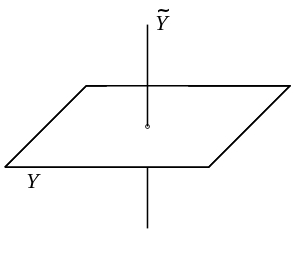
\includegraphics[scale=0.4]{5-1-6.jpg}
\end{enumerate}
\subsubsection{Definition (Orthogonales Komplement)}
Es sei $S \subseteq X$. Dann heißt $S^\bot:=\{x\in X\colon\langle x,y \rangle =0\text{ für alle }y\in S\}$
 das \underline{orthogonale Komplement} von $S$ (in X)
\subsubsection{Beispiel}
\numbers
\begin{enumerate}
\item Es ist $\{0\}^\bot=X$ und $X^{\bot}=\{0\}$
\item Im Raum $X=\R^3$ haben wir in \hyperref[2.5.2]{Beispiel \ref*{2.5.2}} nachgewiesen, dass die Gerade $\tilde{Y}:=\R\begin{pmatrix}1 \\1 \\1\end{pmatrix}$ ein Komplement zur Ebene $Y:=\{x\in X, x_1-x_2+x_3=0\}=\R\begin{pmatrix}1\\1\\0\end{pmatrix}+\R\begin{pmatrix}1\\0\\-1\end{pmatrix}$ ist.
Betrachtet man $\R^3$ als Euklidischen Raum, so ist $\tilde{Y}$ wegen $\left\langle \begin{pmatrix}1 \\1 \\1\end{pmatrix},\begin{pmatrix}1 \\1 \\0\end{pmatrix}\right\rangle=2$ jedoch kein orthogonales Komplement von Y, vielmehr gilt $Y^{\bot}=\R\begin{pmatrix}1 \\-1 \\1\end{pmatrix}$
\end{enumerate}
\subsubsection{Proposition}
\label{5.1.9}
Für jedes $S\subseteq X$ ist $S^{\bot}$ ein Unterraum von $X$ mit $(\spann S)\cap S^{\bot}=\{0\}$.\\
\underline{Beweis}: Es seien $x_1,x_2\in S^{\bot}$ und wir erhalten $\langle \alpha_1 x_1+\alpha_2 x_2,y\rangle=\alpha_1\langle x_1,y\rangle+\alpha_2\langle x_2,y\rangle=0$ für alle $\alpha_1,\alpha_2\in\K$ $y\in S$ dies garantiert $\alpha_1 x_1+\alpha_2 x_2\in S^{\bot}$ und $S^{\bot}$ ist ein linearer Raum.
Weiter sei $x\in\ S^{\bot}$ und $x\in \spann ~S$, d.h. $x=\sum_{i=1}^n \xi_i x_i$ mit Koeffizienten $\xi_i\in \K$ und $x_i\in S$. Dies impliziert $\langle x,x\rangle=\langle \sum_{i=1}^n \xi_i x_i,x\rangle=\sum_{i=1}^n\xi_i \underbrace{\langle x_i,x\rangle}_{=0\text{ weil }x\in S^{\bot}}=0$ und folglich $x=0$.
\subsubsection{Satz}
\label{5.1.10}
Ist $\dim X<\infty$ und $Y$ ein Unterraum von $X$, so gilt
\alphabet
\begin{enumerate}
\item $X=Y\oplus Y^{\bot}$
\item $(Y^{\bot})^{\bot}=Y$
\item $\dim X=\dim Y+\dim Y^{\bot}$
\end{enumerate}
\underline{Beweis (a)}: $Y\cap Y^{\bot}=\{0\}$ gilt nach \hyperref[5.1.9]{Proposition \ref*{5.1.9}}. Es bleibt $X=Y\oplus Y^{\bot}$ zu zeigen. Zu jedem $x\in X$ muss es also $y\in Y$ und $y^{\bot}\in Y^{\bot}$ mit $x=y+y^{\bot}$ geben. Ist $\{y_1, \dots,y_n\}$ eine Orthonormalbasis von $Y$, so definieren wir
\[y:=\sum_{i=1}^m \langle x,y_i\rangle \cdot y_i,\qquad y^{\bot}:=x-y\text{ usw.}\]
\subsubsection{Definition (Orthogonal- und Orthonormalbasis)}
Eine Familie $\mathcal{S} \subseteq X$ heißt
\alphabet
\begin{enumerate}
\item \underline{orthogonal}, falls $\langle x,y\rangle=0$, für alle $x,y\in \mathcal{S}$ $x\neq y$
\item \underline{orthonormal}, falls $\langle x,y\rangle=\begin{cases}1,x=y\\0,x\neq y\end{cases}$, für $x,y\in \mathcal{S}$
\end{enumerate}
Eine Orthogonal- bzw. Orthonormalbasis von X ist eine orthogonale bzw. orthonormale Basis von X.\\
Jede orthonormale Familie ist auch orthogonal.
\subsubsection{Beispiel}
\label{5.1.12}
\numbers
\begin{enumerate}
\item Die Standardbasis $\epsilon_n=\{e_1,\dots,e_n\}$ aus \hyperref[standardbasis]{Beispiel \ref*{standardbasis}} ist eine Orthonormalbasis des Euklidischen Raums $\R^n$ wie auch des unitären Raums $\Co^n$.
\item Die Legendre Polynome $p_n\in P(\R)$, $p_n(t)=\frac{1}{2^n n!} \frac{d^n}{dt^n} (t^2-1)^n$ für $n\in\N_0$ definieren eine orthogonale Familie $\{p_n\}_{n\in\N_0}$ bzgl. dem inneren Produkt (\hyperref[5.1b]{$5.1b$}) aus \hyperref[5.1.6]{Beispiel \ref{5.1.6}(2)} mit $\omega(t)=1$ auf $[-1,1]$
\item Wir definieren die trigonometrischen Funktionen $c_n,s_n\colon[-\pi,\pi]\rightarrow\R$, $c_n(t):=cos(nt)$, $s(t):=sin(nt)$ mit $n\in\N_0$. Dann ist $\mathcal{S}:=\{c_n\}_{n\in\N_0} \cup \{s_n\}_{n\in\N}$ eine orthogonale Familie in $C([-\pi,\pi],\R)$ bezüglich (\hyperref[5.1b]{$5.1b$}) mit $\omega(t)=1$ auf $[-\pi,\pi]$.
\end{enumerate}
\subsubsection{Proposition}
Jede orthogonle Familie $\mathcal{S}\subseteq X$ mit $0\notin\mathcal{S}$ ist linear unabhängig.\\
\underline{Beweis}: Es sei $\{x_1,\dots,x_n\}$ eine endliche Teilfamilie von $\mathcal{S}$ und $\sum_{j=1}^n \xi_j x_j =0$ mit Koeffizienten $\xi_j\in\K$.
Dann resultiert $0=\langle 0,x_k\rangle=\langle\sum_{j=1}^n\xi_j x_j,x_k\rangle=\sum_{j=1}^n \xi_j \langle x_j,x_k\rangle=\xi_k\langle x_j,x_k\rangle$ für alle $1\leq k\leq n$. Wegen $x_k\neq 0$ folgt $\xi_k=0$.\\
Vorteil von Orthonormalbasen: Koordinaten einfach berechenbar
\subsubsection{Proposition}
Ist $\{x_1,\dots,x_n\}$ eine Orthonormalbasis von $X$ so gilt $x=\sum_{j=1}^n \langle x,x_j\rangle x_j$ für alle $x\in X$.\\
\underline{Beweis}: Da $\{x_1,\dots,x_n\}$ orthonormal ist, gilt $\langle x_j,x_k\rangle=\delta_{jk}$ für $1\leq j,k\leq n$. Die Koeffizienten $\xi_j\in\K$ eines beliebigen $x=\sum_{j=1}^n\xi_j x_j \qquad \xi_k=\sum_{j=1}^n\xi_k \underbrace{\langle x_j,x_k\rangle}_{\delta_{jk}}=\langle\sum_{j=1}^n\xi_j x_j,x_k\rangle=\langle x,x_k\rangle$\\
Berechnung von Orthogonal- bzw. Orthonormalbasis aus einer gegebenen Basis: Orthogonalisierungsverfahren von Gram-Schmidt:

\numbers
\begin{enumerate}
\setcounter{enumi}{-1}
\item Es sei eine linear unabhängige Familie $\mathcal{S}:=\{x_1,x_2,x_3,\dots\}$ gegeben auf $X$ mit innerem Produkt $\langle \cdot,\cdot\rangle$
\item Setze $y_1:=x_1$
\item Für $k\geq 1$ definiere
\[\phantomsection\label{5.1c}(5.1c)\ y_{k+1}:=x_{k+1}-\sum _{j=1}^k \frac{\overline{\langle y_j,x_{k+1}\rangle}}{\langle y_j,y_j\rangle}y_j\]
für alle $k\in \mathbb{N}$ solange $x_{k+1}\in\mathcal{S}$.  Wir erhalten aus $\{x_1,x_2,\cdots \}$ eine Familie orthogonaler Vektoren $\{y_1,y_2,\cdots \}=\mathcal{Y}$ und normiert man die Elemente von $\mathcal{Y}$ gemäß
\[\phantomsection\label{5.1d}(5.1d)\ z_k:=\frac{1}{\|y_k\|}y_k,\]
so erhalten wir sogar eine orthonormale Familie.
\end{enumerate}
\subsubsection{Satz}
\label{5.1.15}
Jeder endliche-dimensionale lineare Raum mit innerem Produkt hat eine Orthonormalbasis.\\
\underline{Beweis}: Nach \hyperref[2.4.8]{Satz \ref{2.4.8}} besitzt $X$ eine Basis $\{x_1,\cdots ,x_n\}$.  Auf diese wenden wir obiges Gram-Schmidt-Verfahren an: Es sei $y_1:=x_1$, $y_{k+1}$ für $1\leq k\leq n$ durch \hyperref[5.1c]{$(5.1c)$} gegeben und $\{y_1,\cdots ,y_k\}$ bereits orthogonal.  Wir erhalten dann
\[\langle y_i,y_{k+1}\rangle \stackrel{\hyperref[5.1c]{(5.1c)}}{=}\left\langle y_i,x_{k+1}-\sum _{j=1}^k\frac{\overline{\langle y_j,x_{k+1}}}{\langle y_j,y_j\rangle}y_j\right\rangle = \langle y_i,x_{k+1}\rangle - \left\langle y_i,\sum _{j=1}^k \frac{\overline{\langle y_j,x_{k+1}}}{\langle y_j,y_j\rangle}y_j\right\rangle\]
\[\langle y_i,x_{k+1}\rangle -\sum _{j=1}^k\frac{\langle y_j,x_{k+1}\rangle}{\langle y_j,y_j\rangle}\overbrace{\langle y_i,y_j\rangle}^{\delta_{ij}}\]
\[\langle y_i,x_{k+1}\rangle -\langle y_i,x_{k+1}\rangle = 0\]
dass $y_i$ für alle $1\leq i\leq k$ orthogonal auf $y_{k+1}$ ist.  Wir haben also induktiv eine orthogonale Familie $\{y_1,\cdots ,y_k,y_{k+1}\}$ erzeugt.  Demnach ist $\{y_1,\cdots y_n\}$ eine Orthogonalbasis von $X$.  Die gesuchte Orthonormalbasis $\{z_1,\cdots ,z_n\}$ ergibt sich aus \hyperref[5.1d]{$(5.1d)$}.
\subsubsection{Beispiel (Legendre-Polynome)}
Aufgrund von \hyperref[2.4.4]{Beispiel \ref{2.4.4}} sind die Monome $\mathcal{M}_3:=\{m_0,m_1,m_2,m_3\}$ eine Basis von $P_3(\mathbb{R})$.  Verwenden wir auf $P_3(\R)$ nun das innere Produkt (vgl. \hyperref[5.1b]{$(5.1b)$})
\[\langle p,q\rangle := \int _{-1}^1 p(t)q(t)dt,\]
so ist $\mathcal{M}_3$ wegen $\langle m_k,m_l\rangle = \dfrac{1-(-1)^{k+l+1}}{1+k+l}$ jedoch keine Orthogonalbasis.  Um eine solche zu bestimmen, wenden wir das Gram-Schmidt-Verfahren an.  Zunächst sei dazu $p_0=m_0$ und wegen
\[\langle p_0,m_1\rangle = 0,\ \langle p_0,m_2\rangle = \frac{2}{3},\ \langle p_0,m_3\rangle = 0\]
erhalten wir $p_1=m_1-\dfrac{\langle p_0,m_1\rangle}{\langle p_0,p_0\rangle}p_0=m_1$, also $p_1(t)=t$.  Mittels der Beziehungen
\[\langle p_1,m_2\rangle =0,\ \langle p_1,m_3\rangle =\frac{2}{5}\]
ist weiter $p_2=m_2-\dfrac{\langle p_0,m_2\rangle}{\langle p_0,p_0\rangle}p_0-\dfrac{\langle p_1,m_2\rangle}{\langle p_1,p_1\rangle}p_1=m_2-\dfrac{\langle p_0,m_2\rangle}{\langle p_0,p_0\rangle}p_0$, also $p_2(t)=t^2-\frac{1}{3}$.  Ebenso erhält man $p_3(t)=t^3-\frac{3}{5}t$ und hieraus ergibt sich die Orthonormalbasis $\{q_0,q_1,q_2,q_3\}$ des $P_3(\R)$ mit
\[q_0(t)\equiv\sqrt{\frac{1}{2}},\ q_1(t)=\sqrt{\frac{3}{2}}t,\ q_2(t)=\frac{3}{2}\sqrt{\frac{5}{2}}(t^2-\frac{1}{3}),\ q_3(t)=\frac{5}{2}\sqrt{\frac{7}{2}}(t^3-\frac{3}{5}t)\]
Fordert man nicht die Normierung $\langle q_k,q_k\rangle = 1$, sondern $q_k(1)=1$, so ergibt sich durch Multiplikation der $p_k$ mit einem geeigneten Faktor, dass
\[q_0(t)\equiv 1,\ q_1(t)=t,\ q_2(t)=\frac{1}{2}(3t^2-1),\ q_3(t)=\frac{1}{2}(5t^3-3t);\]
dies sind die Legendre-Polynome aus \hyperref[5.1.12]{Beispiel \ref{5.1.12}(2)}
\subsection{Adjungierte Abbildungen}
Sei $X$ ein linearer Raum über $\K$ mit innerem Produkt $\langle \cdot ,\cdot\rangle$.  Eine lineare Abbildung $S\colon X\rightarrow \K$ heißt \underline{Funktional}.  Mit gegebenem $y\in X$ definieren wir das Funktional $y'\colon X\rightarrow \K$ durch
\[\phantomsection\label{5.2a}(5.2a)\ y'(x)\colon =\langle x,y\rangle\text{ für alle } x\in X\]
Aufgrund von \hyperref[5.1.1]{Definition \ref{5.1.1}(i)} gilt nämlich $y'(\alpha _1x_1+\alpha _2x_2)=\langle \alpha _1x_1+\alpha _2x_2,y\rangle = \alpha _1\langle x_1,y\rangle +\alpha _2\langle x_2,y\rangle = \alpha _1 y'(x_1)+\alpha _2 y'(x_2)$ für alle $\alpha _1,\alpha _2\in \K ,\ x_1,x_2\in X$, also $y'\in L(X,\K)$
\subsubsection{Satz (Riesz'scher Darstellungssatz)}
\label{5.2.1}
Ist $\dim X<\infty$, so gibt es zu jedem Funktional $S\in L(X,\K)$ ein eindeutiges $y\in X$ mit $Sx=\langle x,y\rangle$ für alle $x\in X$, d.h. $S=y'$.\\
\underline{Beweis}: Nach \hyperref[5.1.15]{Satz \ref{5.1.15}} gibt es eine Orthonormalbasis $\{x_1,\cdots ,x_n\}$ von $X$.
\Romannum
\begin{enumerate}
\item \underline{Existenz}: Zu beliebig gegebenem $S\in L(X,\K)$ sei
\[\phantomsection\label{5.2b}(5.2b)\ y\colon = \sum _{i=1}^n \overline{Sx_i}x_i\in X\]
und es gilt
\[\langle x_j,y\rangle \stackrel{\hyperref[5.2b]{(5.2b)}}{=} \left\langle x_j,\sum _{i=1}^n\overline{Sx_i}x_i\right\rangle =\sum _{i=1}^n \overline{\overline{Sx_i}}\overbrace{\langle x_j,x_i\rangle}^{\delta_{ij}}=Sx_j\text{ für }1\leq j\leq n\]
Damit stimmen $S$ und $y'$ auf einer Basis von $X$ überein, weshalb \hyperref[lfortsetzung]{Satz \ref{lfortsetzung}(a)} sofort $S=y'$ garantiert.
\item \underline{Eindeutigkeit}: Um nachzuweisen, dass obiges $y$ aus \hyperref[5.2b]{$(5.2b)$} eindeutig bestimmt ist, erfülle auch $z\in X$ die Beziehung $Sx=\langle x,y\rangle = \langle x,z\rangle $ für alle $x\in X$.  Dies impliziert $\langle x,y-z\rangle = 0$ für alle $x\in X$ und damit $y-z=0$
\end{enumerate}
Nun seien $T\in L(X)$, $y\in X$.  Wir definieren $S_y\colon X\rightarrow \K$
\[S_yx\colon =\langle Tx,y\rangle\]
und es folgt sofort $S_y\in L(X,\K)$.  Bei festem $T$ gibt es nach \hyperref[5.2.1]{Satz \ref{5.2.1}} zu jedem $y\in X$ ein eindeutiges $y_0\in X$ mit $S_yx=\langle x,y_0\rangle$ für alle $x\in X$.  Wir bezeichnen diese Zuordnung $y\mapsto y_0$ mit $T'$ und die entsprechende Abbildung $T' \colon X\rightarrow X$ ist festgelegt durch
\[\langle Tx,y\rangle = \langle x,T' y\rangle\text{ für alle }x,y\in X\]
Gegeben $T=L(X)$, $y\in X$.  Wir definieren:
\[S_yx:=\langle Tx,y\rangle\]
und mittels \hyperref[3.1a]{$(3.1a)$}, sowie \hyperref[5.1.1]{Definition \ref{5.1.1}$(i)$} folgt sofort $S_y\in L(X,\K)$.  Bei festen $T\in L(X)$ gibt es nach \hyperref[5.2.1]{Satz \ref{5.2.1}} dann ein eindeutig bestimmtes $y_0\in X$mit $S_yx=\langle x,y_0\rangle$.  Wir bezeichnen diese Zuordnung $y\mapsto y_0$ mit $T'$ und die Abbildung $T'\colon X\rightarrow X$ ist festgelegt durch $\langle Tx,y\rangle=\langle x,T'y\rangle$ für alle $x,y\in X$.  Aufgrund von \hyperref[5.1.1]{Definition \ref{5.1.1}} erhalten wir mit beliebigen $x_1,x_2\in X$,$\alpha _1,\alpha _2\in \K$, dass
\[\langle x,T'(\alpha _1x_1+\alpha _2x_2)\rangle =\langle Tx,\alpha _1x_1+\alpha _2x_2\rangle = \overline{\alpha _1}\langle Tx,x_1\rangle +\overline{\alpha _2}\langle Tx,x_2\rangle=\overline{\alpha _1}\langle x,T'x_1\rangle + \overline{\alpha _2}\langle x,T'x_2\rangle\]
\[\langle x,\alpha _1T'x_1+\alpha _2T'x_2\rangle\]
Damit ist $T'\in L(X)$.
\subsubsection{Definition (adjungierte Abbildung)}
Die zu $T\in L(X)$ \underline{adjungierte Abbildung} $T'\in L(X)$ ist definiert durch
\[\phantomsection\label{5.2c}(5.2c)\ \langle Tx,y\rangle = \langle x,T'y\rangle \text{ für alle } x,y\in X\]
Man beachte, dass $T'$ von konkret auf $X$ verwendete inneren Produkt abhängt.
\subsubsection{Bemerkung}
Direkt aus \hyperref[5.2c]{$(5.2c)$} folgt
\numbers
\begin{enumerate}
\item Die Abbildung $\cdot '\colon L(X)\rightarrow L(X)$ ist \underline{semilinear}, d.h.
\[(\alpha _1T_1+\alpha _2T_2)'=\overline{\alpha _1}T'_1+\overline{\alpha _2}T'_2\text{ für }\alpha _1,\alpha _2\in \K, T_1,T_2\in L(X)\]
und erfüllt $T''=T$, sowie $(ST)'=T'S'$ für $S,T\in L(X)$
\item Für $T\in GL(X)$ ist auch $T'\in GL(X)$ mit
\[(T')^{-1}=(T^{-1})'\]
\end{enumerate}
\subsubsection{Beispiel (Transponierte)}
Es sei $X=\R ^n$ (Euklidisch) ausgestattet mit der Standardbasis $\mathcal{E}_n=\{e_1,\cdots ,e_n\}$ und $A\in \R ^{n\times n}$ die darstellende Matrix von $T\in L(X)$, d.h. $Tx=Ax$ für alle $X\in \R ^n$.  Bezeichnet dann $A'\in \R ^{n\times n}$ die darstellende Matrix von $T'$, so ist
\[a'_{ij}=\left\langle e_i,\begin{pmatrix}a'_{1j}\\ \vdots \\ a'_{nj}\end{pmatrix}\right\rangle = \langle e_i,T'e_j\rangle\stackrel{\hyperref[5.2c]{(5.2c)}}{=}\langle Te_i,e_j\rangle =\left\langle \begin{pmatrix}a_{1i}\\ \vdots \\ a_{ni}\end{pmatrix},e_j\right\rangle = a_{ij} \text{ für alle }1\leq i,j\leq n.\]
Folglich ist die adjungierte Abbildung $T'$ in Euklidischen Räumen gerade durch die Transponierte $A'=A^T$ gegeben (vergleiche \hyperref[3.2.3]{Beispiel \ref{3.2.3}}).
\subsubsection{Beispiel (Hermite'sche)}
\label{5.2.5}
Im unitärer Raum $\Co ^n$ mit seiner Standardbasis $\mathcal{E}_n$ ergibt sich entsprechend:
\[\overline{a'_{ij}}=\left\langle e_i,\begin{pmatrix}a'_{1j}\\ \vdots \\ a'_{nj}\end{pmatrix} e_i,T'e_j\right\rangle \stackrel{\hyperref[5.2c]{(5.2c)}}{=}\langle Te_i,e_j\rangle = \left\langle \begin{pmatrix}a_{1i}\\ \vdots \\ a_{ni}\end{pmatrix},e_j\right\rangle=a_{ji}\text{ für alle } 1\leq i,j\leq n\]
und folglich $a'_{ij}=\overline{a_{ji}}$.  Für die adjungierte Abbildung in unitären Räumen ist also $A'=A^*$ mit der sogenannten \underline{Hermite'schen}
\[A^*=\overline{(A^T)}=(\overline{a_{ji}})_{1\leq i,j\leq n}\]
\subsubsection{Satz}
Ist $\dim X<\infty$ und $T\in L(X)$, so gilt
\[N(T')=R(T)^\bot\ \ \mathrm{rk}T=\mathrm{rk}T'\]
\underline{Beweis}: Wir erhalten
\[N(T')=\{x\in X\colon T'x=0\}=\{x\in X\colon \langle y, T'x\rangle =0\text{ für alle }y\in X\}\]
\[\stackrel{\hyperref[5.2c]{(5.2c)}}{=}\{x\in X\colon \langle Ty,x\rangle =0\text{ für alle } y\in X\}=R(T)^\bot\]
Mit \hyperref[5.1.10]{Satz \ref{5.1.10}(c)}, der eben gezeigten Aussage und \hyperref[dimension]{Satz \ref{dimension}}
\[\mathrm{rk}T=\dim R(T)=\footnotemark\dim X-\dim R(T)^\bot =\dim  X-\dim N(T')=\dim R(T')=\mathrm{rk}T'\]
\footnotetext{gilt wegen: $X=Y\oplus Y^\bot\\ \dim X=\dim Y+\dim Y^\bot$}
\subsection{Sebstadjungierte Abbildungen}
Wieder sei $X$ ein linearer Raum mit inneren Produkt $\langle \cdot ,\cdots \rangle$
\subsubsection{Definition (Selbstadjungiert)}
Eine Abbildung $T\in L(X)$ heißt \underline{selbstadjungiert}, falls gilt $T=T'$, d.h.
\[\phantomsection\label{5.3a}(5.3a)\langle Tx,y\rangle =\langle x,Ty\rangle \text{ für alle }x,y\in X\]
\subsubsection{Beispiel (Euklidischer Raum)}
Auf dem Euklidischen Raum $\R ^n$ ist eine Abbildung $T\in L(X)$ genau dann selbstadjungiert, falls ihre darstellende Matrix $T_{\mathcal{E}_n}=A$ \underline{symmetrisch} ist, d.h. $A=A^T$
\[\text{z.B.}\ \begin{pmatrix}1 & 2\\ 2 & 1\end{pmatrix},\begin{pmatrix}1 & 3\\ 3 & 2\end{pmatrix}, \begin{pmatrix}1 & 2\\ 3 & 4\end{pmatrix}\text{ nicht.}\]
\subsubsection{Beispiel (unitärer Raum)}
In einem unitären Raum $\Co ^n$ ist $T\in L(\Co ^n)$ dann und nur dann selbstadjungiert, wenn $A=T_{\mathcal{E}_n}$ Hermite'sch ist (vergleiche \hyperref[5.2.5]{Beispiel \ref{5.2.5}}), d.h. $A=A^*$.
\addtocounter{subsubsection}{1}
\subsubsection{Satz}
Es sei $\dim X<\infty$.  Ist $T\in L(X)$ selbstadjungiert, so gilt:
\alphabet
\begin{enumerate}
\item $\sigma (T)\subseteq \R$
\item Es gibt eine Orthonormalbasis von $X$ aus Eigenvektoren von $T$
\end{enumerate}
\subsubsection{Bemerkung}
Auf Matrizen bezogen besagt dies gerade, dass symmetrische und Hermite'sche Matrizen reelles Spektrum haben und der Raum $\K ^n$ eine Orthonormalbasis aus Eigenvektoren besitzt.
\underline{Beweis}: 
\begin{enumerate}
\item Es sei $\lambda \in \K$ ein Eigenwert von $T$ mit zugehörigen Eigenvektor $x\in X$.  Da $T$ selbstadjungiert ist, gilt
\[\lambda \langle x,x\rangle = \langle \lambda x,x\rangle \stackrel{\hyperref[4.2a]{(4.2a)}}{=}\langle Tx,x\rangle = \langle x,Tx\rangle \stackrel{\hyperref[4.2a]{(4.2a)}}{=} \langle x,\lambda x\rangle = \overline{\lambda}\langle x,x\rangle\]
und wegen $x\not=0$ folgt $\lambda =\overline{\lambda}$, also $\lambda \in \R$.
\item Induktion über $n=\dim X$.  Für $n=1$ ist nichts nachzuweisen.  Für $n>1$ gilt den Fundamentalsatz der Algebra
\[\chi _T(t)=\prod _{i=1}^n(\lambda _i-t)\text{ mit }\lambda _i\in \Co\]
und wegen \hyperref[4.3.3]{Satz \ref{4.3.3}} ist jedes $\lambda _i$ Eigenwert von $T$;
Aussage (a) garantiert sogar $\lambda _i\in \R$.  Es sei nun $x_1$ ein normierter Eigenvektor zu $\lambda _1$ und $X_1=(\spann \{x_1\})^\bot$.  Mittels \hyperref[5.1.10]{Satz \ref{5.1.10}(c)} ist dann $\dim X_1=n-1$.  Für jedes $x\in X_1$ ist dann
\[\langle x_1,Tx\rangle \stackrel{\hyperref[5.3a]{(5.3a)}}{=}\langle Tx_1,x\rangle \stackrel{\hyperref[4.2a]{(4.2a)}}{=}\lambda _1\overbrace{\langle x_1,x\rangle}^0=0\]
d.h. $Tx\in X_1$.  Wir haben damit gezeigt, dass $X_1$ invariant unter $T$ ist.  Damit induziert $T\in L(X)$ eine selbstadjungierte Abbildung $T_1\colon =T\mid _{X_1}\in L(X_1)$.  Nach Induktionsvoraussetzung gilt es eine Orthonormalbasis $\mathcal{X}_1\colon =\{x_2,\cdots ,x_n\}$ von $X_1$ aus nomierten Eigenvektoren $x_i$ von $T$.  Da jeder Eigenvektor von $T_1$ auch Eigenvektor von $T$ ist, muss $\{x_1,x_2,\cdots ,x_n\}$ eine Orthonormalbasis von $X$ sein.
\end{enumerate}
\subsubsection{Korollar}
Jede selbstadjungierte Abbildung ist diagonalisierbar.
\underline{Beweis}: Wähle Basis aus Eigenvektoren.
\end{document}
